\documentclass[oneside]{article}
\usepackage{fullpage}
\usepackage[pdftex]{graphicx}
\DeclareGraphicsExtensions{.png,.pdf}
\graphicspath{{images/}}
\usepackage[dvipsnames,usenames]{color}
\usepackage{hyperref}
\usepackage{verbatim}
\usepackage[format=plain,font=small]{caption}
\usepackage[small]{titlesec}
\usepackage[round,sectionbib]{natbib}
\usepackage{amstext}
\usepackage{setspace}
\bibliographystyle{plainnat}
\renewcommand\rmdefault{bch}
\linespread{1.07} 

\newcommand\amin{\text{minor}}
\newcommand\amaj{\text{major}}

\begin{document}
\doublespacing
\title{Glyph-maps for Visually Exploring Temporal Patterns in Climate Data and Models}
\author{Hadley Wickham$^1$, Heike Hofmann$^2$, Charlotte Wickham$^3$, Dianne Cook$^2$\\
$^1$Department of Statistics, Rice University\\
$^2$Department of Statistics, Iowa State University\\
$^3$Department of Statistics, Oregon State University}
\date{}

% Remove words like "obvious", "challenge", "scratched the surface"
% Make data URLs references
% Do we have different aspect ratios between the different US maps?
% Check where data is described, just use key names given in the description at beginning of paper

% Found data: http://www.esrl.noaa.gov/psd/data/gridded/data.HADCRUT2.html
%     air.mon.anom.nc, var adj, this is 5x5 degree grid, a bit sparse
% Or: http://www.esrl.noaa.gov/psd/data/gridded/data.gisstemp.html
% air.2x2.mon.anom.land.nc 250k smooth data, is on a 2x2 grid

% Drawing trend lines on map
%   - How to
%   - Comparison to coloring slope
%   - Reference to Grinstein icon plots
% Pickett RM and Grinstein GG (1988). Iconographics 
% displays for visualizing multidimensional data. 
% In Proc. IEEE Conference on Systems, Man, and Cybernetics, pages 514-19.
% Note the later work on metaphoric data display, garbage work!
%   - Alexander Gribov's work http://rosuda.org/software/Gauguin/gauguin.html

%   - Spatial star plots by Andrews http://www.udallas.edu:8080/~andrews/software/software.html
%   - Look at what Bertin does
%
% Interactive graphics
% Data processing
%
% Perhaps the GHCN data? Not gridded
% NOAA data, almost grid, but over ocean, so maps more tricky
% NARCAP from NCAR?
% Fill in with NASA data, to start, try to put new data for final version
\maketitle

% re-work equations, to incorporate scale, and interaction, use spatial location letter and time/var letters

% overlay legends on the plots?

\begin{abstract}

The multivariate spatio-temporal nature of climate data makes it difficult to draw all of the aspects simultaneously. This paper describes the conceptualization and construction of a type of display, a glyph-map, that has been used infrequently for climate data. Glyph-maps are a specialization of multivariate glyph plots. Each spatial location is displayed with one glyph that represents the multiple measurements, recorded over time, at that location. Glyph-maps allow the discovery of both local and global structure, with a particular focus on temporal relationships. They provide alternatives to colored, facetted maps, or statistical summaries such as principal components. With the new conceptualization, developing interactive versions of glyph-maps will be easier, and it will be simpler to explore the perceptual effects of different scales. The methods are developed for rectangularly gridded data, but with some clever processing, which is explained, it is possible get good glyph-maps of irregularly gridded data. Guides, and reference marks, for different types of glyphs used in the glyph-maps are also discussed.

%Understanding the multiple aspects of climate data is a challenge. There are both spatial and temporal components to examine, and often multivariate dependencies. This paper proposes a new display for climate data: glyph-maps. Glyph-maps are a specialization of multivariate glyph plots; each spatial location is displayed with one glyph that represents the measurements recorded over time at that location. Glyph-maps allow the discovery of both local and global structure, with a particular focus on temporal relationships.

%The instructions for computing and displaying glyph-maps are described, along with the design of reference frames, and the effects of different scaling of the data on perception of structure. The methods are developed for rectangularly gridded data, but with some clever processing, which is explained, it is possible get good glyph-maps of irregularly gridded data.

\end{abstract}

\section{Introduction}

Climate data is composed of multiple variables, such as temperature, ozone, precipitation, and winds, with a spatial and temporal context. The classic display for data of this type is a ``heatmap'', a tiled plot using color to display the value of the variable of interest at each location. When measurements are made at multiple time points it is reasonably common to display the data with small multiples~\citep{tufte:2001}, such as in Figure~\ref{fig:nasa-facet}. In this plot, a separate map is drawn for each month (columns) and year (rows), over a six year period of remotely sensed temperature data above Central America \citep{murrell:2010}. Color is used to display de-seasonalized temperature (residuals from a linear model containing year and month terms), where red is mapped to high values and blue to low. The most noticeable feature is the strong red patch in the equatorial Pacific beginning mid-1997 and tapering out during 1998. This is the El Ni\~no event, a major temperature anomaly (see for example, \citet{trenberth} or \url{http://www.esrl.noaa.gov/psd/enso/enso.description.html}.) More work is required to see more localized patterns, like the cooler land temperatures seen in early years.

To read long-term or localized temporal patterns, this type of plot is cognitively challenging: the reader must play ``spot the difference'' from one small image to another. Large spatial structures such as El Ni\~no are clear but it is very difficult to extract the temporal pattern because it requires mentally differencing the images. Using a movie to render these small multiples can help, but small trends still fail to draw readers' attention and escape unnoticed \citep{simons:gradual}. The \emph{glyph-map} display described in this paper enables easier perception of temporal patterns. 

%% Reproduce all of the icon displays using the fixed glyph code

The glyph-map uses a small glyph, or icon, to represent multiple variables, or time values, at each location. Glyph maps derive from glyph plots, which were initially developed to display multivariate data. One glyph is drawn for each observation in the data set. Types of glyph plots include the star plots \citep{mayr:1877, FD01, kleiner:1981}, the semi-graphic displays \citep{anderson:1960}, and the infamous Chernoff faces \citep{chernoff:1973}. An glyph is produced by mapping each variable to some graphical feature, such as the length of a line, curvature of the mouth, or size of the face. 

Figure~\ref{fig:nasa-glyph} shows the glyph-map equivalent of Figure~\ref{fig:nasa-facet}: each location is represented by a small time series glyph of de-seasonalized temperature. The darker grey in the background represents the land mass of the study region. Because the data is de-seasonalized, the primary visible structure is still El Ni\~no -- it is both a temporal anomaly and a spatial phenomenon. It can be recognized by the bump in the middle of the series of the equatorial Pacific region. Other temporal features are visible from the many time series. Temperatures are generally more varied over land, than sea. A few locations have dramatic jumps in temperature in the later years.%, all in high elevation areas, along the Andes and the Sierra Madre Occidental in Mexico. 

The glyph-map can also be thought of as a small multiple display. The primary comparison is different from the facetted heatmap. Cognitively, elements placed close to each other are more easily and accurately compared \citep{cleveland:1984}. The facetted heatmap, places greater emphasis on comparison between the spatial locations, because these are positioned together, and secondary emphasis on time because these are separated by facets. In the glyph-map, primary emphasis is placed on the temporal comparison, and secondarily on spatial comparison, because facetting is on spatial locations.  

% The most seasonality occurs in north American. Some seasonal effects can also be seen in the Caribbean and in south American locations. Around the equator the temperatures are relatively warm for all seasons. Instead of radially displaying the temperature a glyph can be a regular time series, time displayed horizontally and temperature vertically (right plot). The structure perceived is different with this change in glyph type: locations at the equator have flat series, on land more varied temperatures. 

\begin{figure*}[htbp]
  \centering
  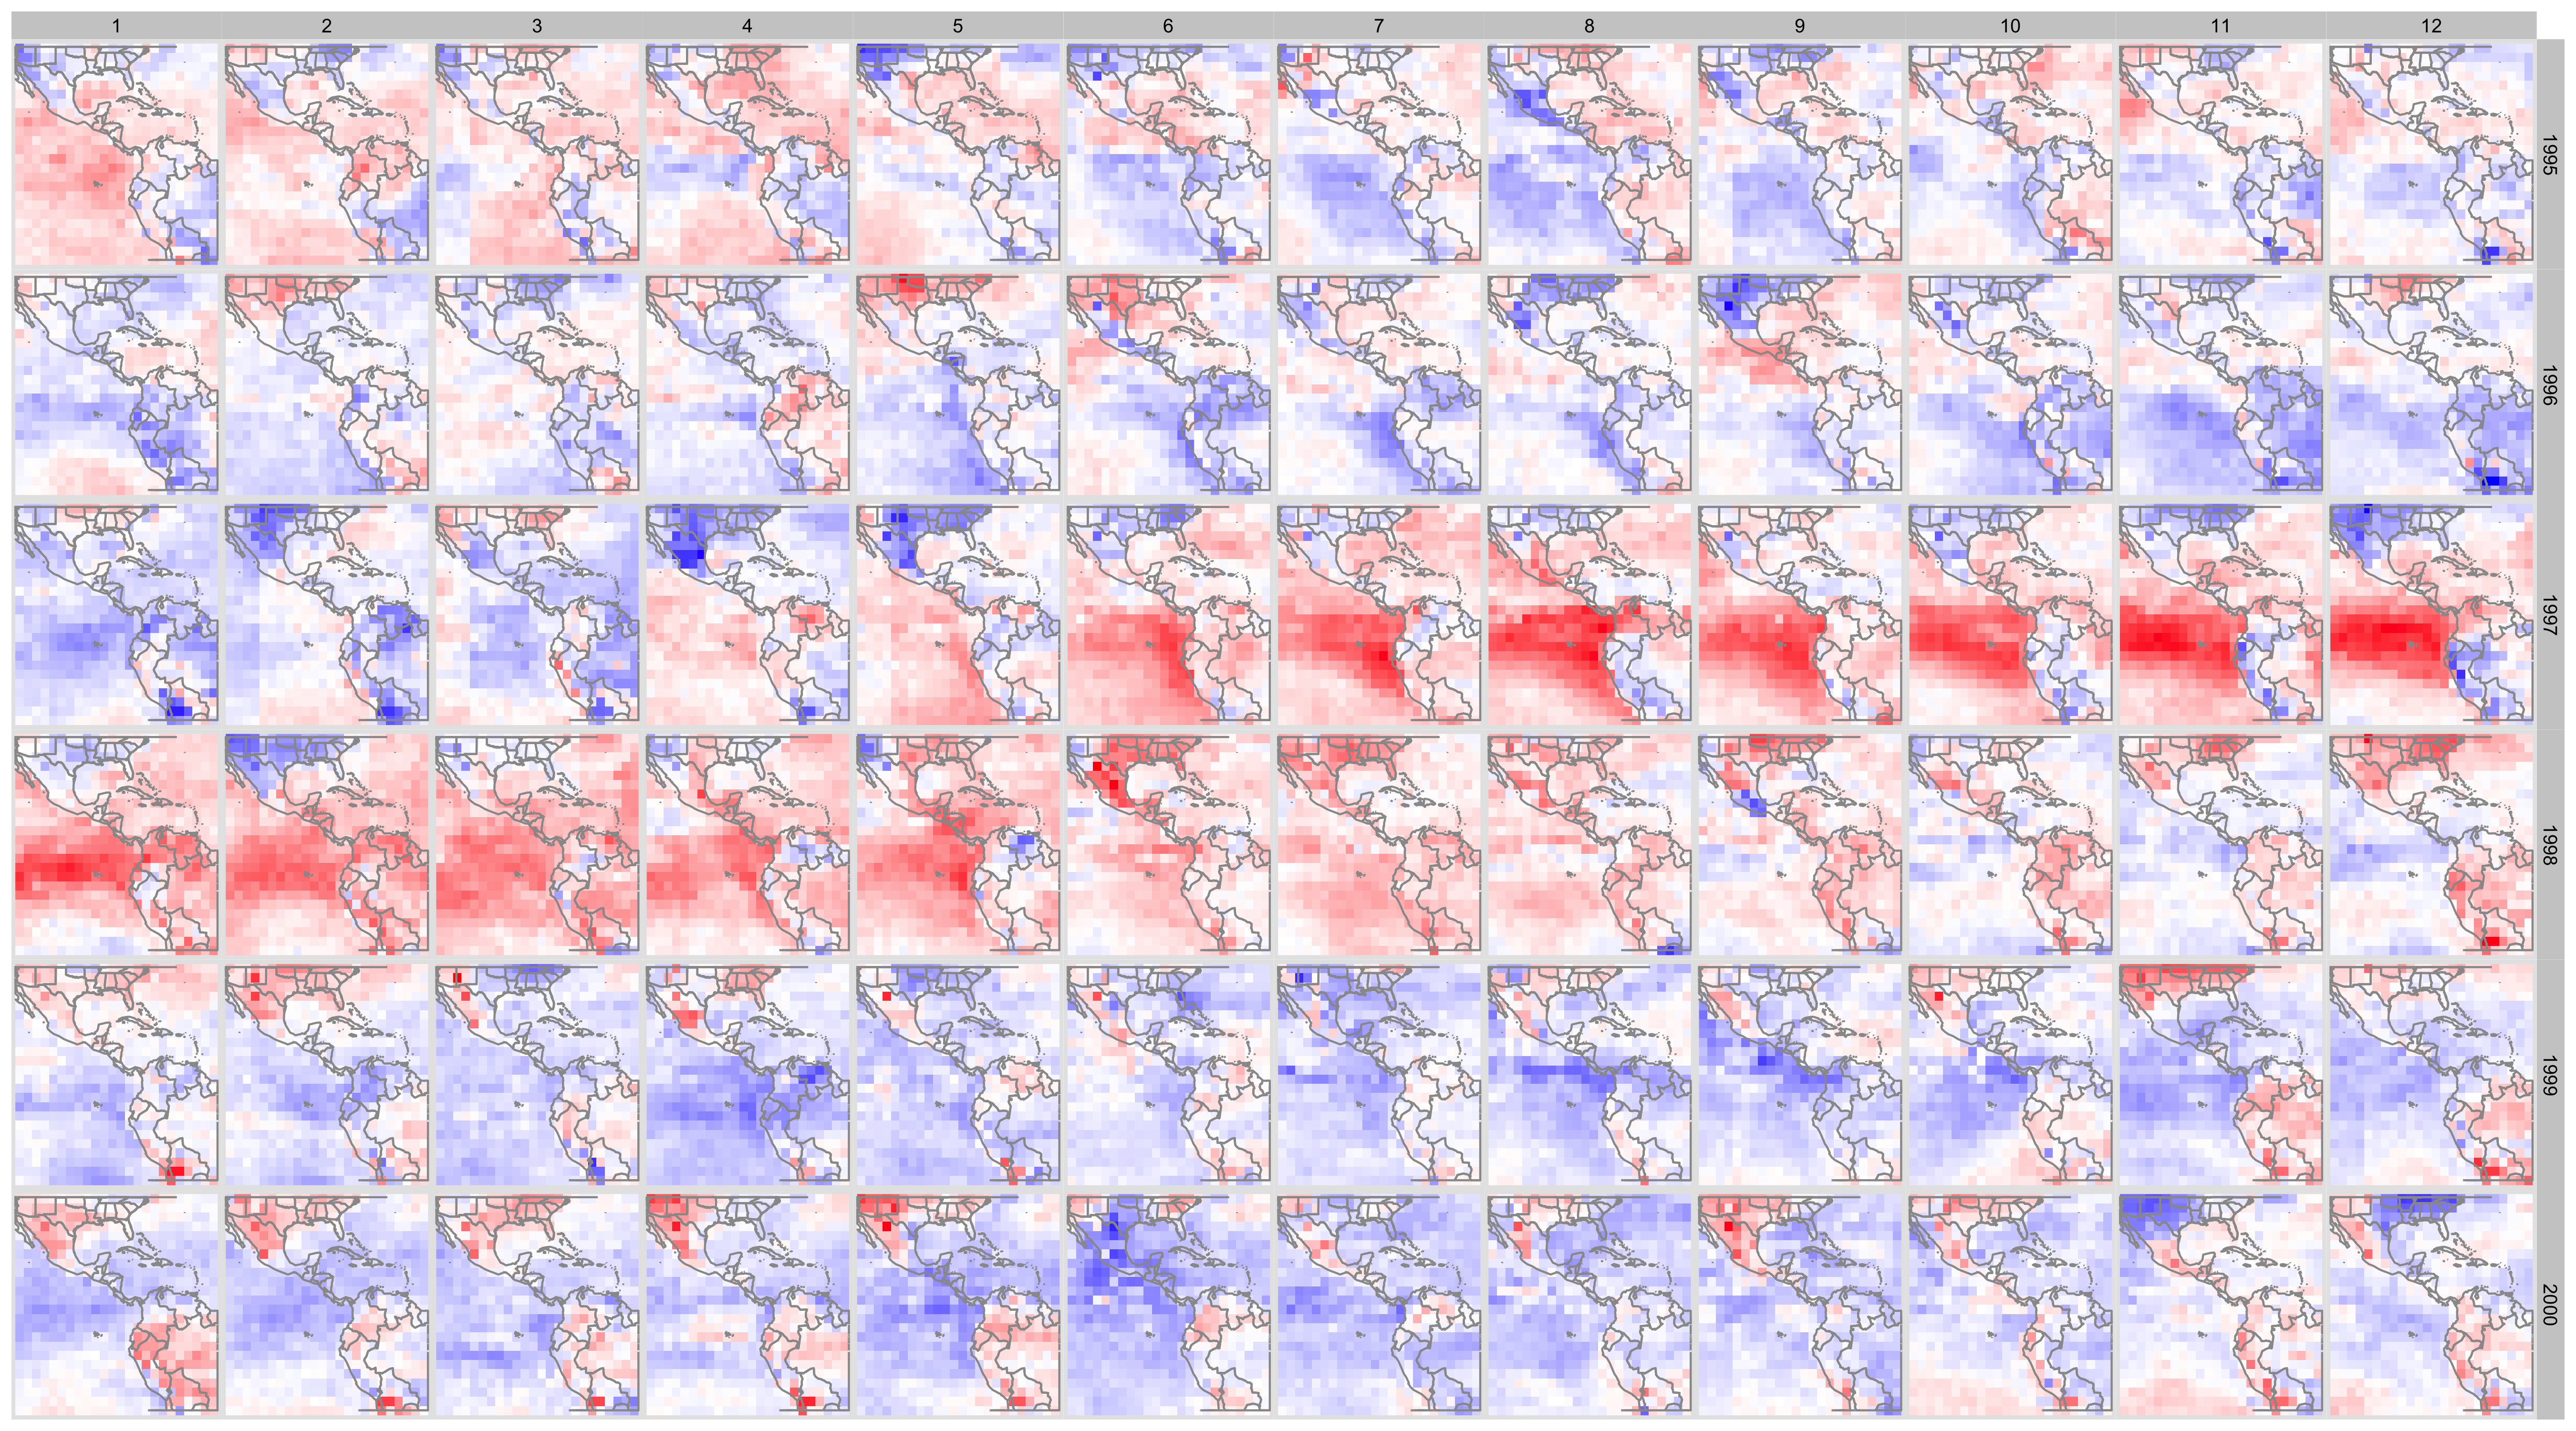
\includegraphics[width=5.5in]{nasa-colored-map.png}
  \caption{Facetted heatmap of de-seasonalized temperature. The dominant feature is the El Ni\~no warming in the southern equatorial region in the last half of 1997 and first half of 1998. Smaller features are only noticeable on closer inspection, or if pointed out: such as the relative warming on the mountain regions in south and north America which are red in all months in the later years.}
  \label{fig:nasa-facet}
\end{figure*}

\begin{figure*}[htbp]
  \centering
  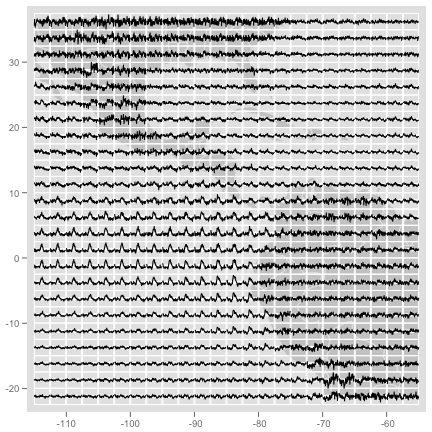
\includegraphics[width=3.5in]{nasa-deseas-glyph}
  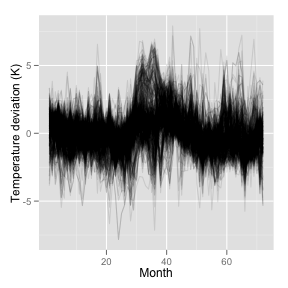
\includegraphics[width=2in]{nasa-deseas-glyph-leg}
  \caption{(Left) Glyph-map of de-seasonalized temperature, to compare with Figure \ref{fig:nasa-facet}. Time series of the six years of monthly temperature are plotted at each spatial grid location. The El Ni\~no appears as a bump in the middle of the time series, in the equatorial Pacific region. Large variations in temperature can be seen in areas over land, while being fairly constant over water. (Right) Glyph-map legend, showing temporal pattern without spatial pattern, giving the scale of the glyphs.}
  \label{fig:nasa-glyph}
\end{figure*}

In general, multivariate glyph displays lack a natural ordering of the glyphs because observations have no ordering. Similarly, there are multiple ways that variables can be mapped to glyph property. It can result in a combinatorial explosion of possible mappings, each producing a display that may emphasize some entirely different features of the data than another mapping. This may have prevented the widespread adoption of glyph displays, despite some proposed ordering solutions \citep{kleiner:1981,hurley:2010}. Using glyphs with space-time data eliminates this issue: glyphs are placed according to the location of the measurement, and variables are ordered by the time they were collected. Additionally, climate data usually has high correlations between nearby locations and times. This imposes a degree of smoothness that gives the plot an appearance of a textured  landscape, making it easier to digest patterns from one glyph to another. Others \citep{pickett:1988} have used glyphs on maps to display multivariate spatial data. This area of work has morphed into the field of metaphorical data displays, which create abstract landscapes of spatial data, a digression from glyph-maps. \citet{gribov:2006} describes the use of glyph-maps for multivariate data also, with emphasis on the graphics software Gauguin. Glyph-maps for spatiotemporal data have been used in several publications \citep{carr:1992,eden:2010,hobbs:2010}. Glyph-maps using arrow glyphs have commonly been used for displaying ocean currents, wind direction and strength, as can be seen in the Figure 8.1 of \citet{IPCC} and a rudimentary time series glyph display can be seen in Figure 9.12. 

Another common approach for displaying spatiotemporal data is to calculate a statistical summary for each location and display these values as single heatmap. For example, to study long-term trends, the slope of a linear model can be calculated at each location and color tiles used to display the slope value over space. This approach is less than exploratory, in the sense that it requires a pre-conceived definition of the relationship of interest, and clean data so that the summary statistic adequately summarizes the pattern. 

Two types of glyph -- lines and stars -- are especially useful for temporal displays. Figure~\ref{fig:templates} displays 12 iconic time series shapes with line- and star-glyphs. The data underlying each glyph is measured at 36 time points. The line-glyphs are   time series plots. The star-glyphs are formed by considering the 36 axes radiating from a common midpoint, and the data values for the row are plotted on each axis relative to the locations of the minimum and maximum of the variable. This is a polar transformation of the line-glyph.

\begin{figure}[htbp]
  \centering
  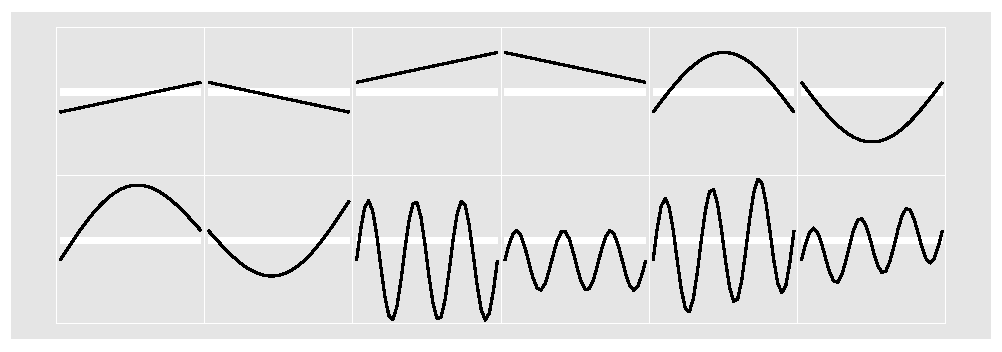
\includegraphics[width=0.5\linewidth]{euclid-to-polar-1}%
  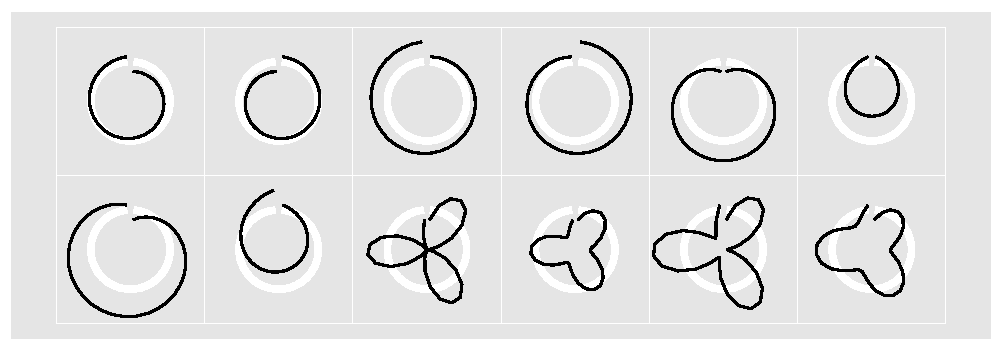
\includegraphics[width=0.5\linewidth]{euclid-to-polar-2}

  \caption{Icon plots for 12 iconic time series shapes (linear increasing, decreasing, shifted, single peak, single dip, combined linear and nonlinear, seasonal trends with different scales, and a combined linear and seasonal trend) in Euclidean coordinates, time series icons (left) and polar coordinates, star plots (right). White reference grids, lines and circles are added to help compare the shapes.}
  \label{fig:templates}
\end{figure}

%Glyph-maps have attributes of both glyphs (stars, faces, profiles, ...), inviting exploration at the global level, and small-multiple time series, allowing local exploration of individual series. Allow to see both geographic context and individual locations simultaneously.

%These displays tend to be particularly effective when printed in large format, as the much higher resolution of print (600 dpi) compared to computer  screen (72-120 dpi) allows for much finer reading. These are high-density data displays in the best tradition of Tufte. Wall size maps are not usually practical during analysis, but are very engaging.

Section~\ref{sec:construction} describes the algorithm used to create glyphs-maps of these two types of glyphs. Section~\ref{sec:perception} discusses their perceptual properties, including the importance of a visual reference grids, and of careful consideration of scale. Large data and the interplay with models and data are discussed in Section~\ref{sec:large-data}. Many spatiotemporal data sets have irregular spatial locations, and Section~\ref{sec:irregular} discusses how glyph-maps can be constructed for this type of data. Three datasets are used for examples:

\begin{quote}
\begin{itemize} \itemsep 0in

\item[EXPO] The ASA 2009 data expo data \citep{murrell:2010} consists
  of monthly observations of several atmospheric variables from the
  International Satellite Cloud Climatology Project. The dataset
  includes observations over 72 months (1995--2000) on a 24 x 24 grid
  (576 locations) stretching from $113.75^{\circ}$W to
  $56.25^{\circ}$W longitude and $21.25^{\circ}$S to $36.25{^\circ}$N
  latitude.

\item[GISTEMP] surface temperature data provided on $2^{\circ}$ x
  $2^{\circ}$ grid over the entire globe, measured monthly
  \citep{GISTEMP} from 1880-2011. Ground station data was de-seasonalized,
  differenced from from the 1951-1980 temperature averages, and
  spatially averaged to obtain gridded temperature anomalies. For the
  purposes of this paper, we extracted the locations corresponding to
  the continental USA.

\item[USHCN] (Version 2) ground station network of historical
  temperatures \citep{USHCN}. Temperatures from 1219 stations on the
  contiguous United States, from 1871 to present.
  
\end{itemize}
\end{quote}
Supplementary material contains the datasets and code to reproduce the plots in this paper.  R 2.13.1 \citep{R} with the packages {\tt ggplot2} \citep{me:ggplot2} and {\tt plyr} \citep{me:plyr} was used. 


\section{Construction}~\label{sec:construction}

%Glyph-maps can be generated with existing graphics software after performing a simple pre-processing step, making them easily accessible to a wide audience. 
To create a glyph-map it is useful to recognize that the glyph-map is a linear mix of two structural components of the data: spatial location and data values. The spatial location is the major positioning component, while the data values are minor adjustments to those positions. For spatiotemporal data, the major components are latitude ($y_{\amaj}$) and longitude ($x_{\amaj}$), and the minor components are time ($x_{\amin}$) and some measurement ($y_{\amin}$), for example, temperature, or predicted temperature. Assuming the minor components are rescaled to $[-1, 1]$, the final coordinates $(x,y)$ on the chart are the linear combination, given by:

\begin{equation}
  \begin{array}{lll}
  x &=& x_{\amaj} + \frac{w}{2} \cdot x_{\amin}\\
  y &=& y_{\amaj} + \frac{h}{2} \cdot y_{\amin}, 
  \end{array}
  \label{coords.eqn}
\end{equation}

\noindent where $w$ and $h$ are scale parameters, setting the width and height of the glyph, respectively. For gridded data, $w$ and $h$ will be the minimum difference between neighboring spatial locations to make use of the resolution of the major components. 

This way of thinking of the glyph-map is convenenient for several reasons. The first is that it moves the plots beyond the small multiples, many little plots, approach. That provides flexibility to cover large spatial domains using potentially tiny glyphs. A second, and major, reason is that with this approach they can then be readily made to be interactive. Different variables can be swept into, and out of, the minor axes using mouse motion by varying $w$ and $h$ proportional to mouse movement. Interactive glyph-maps were used to explore the EXPO data using  GGobi \citep{swayne:2003}, and then later reproduced in publication quality resolution using {\tt ggplot2} \citep{me:ggplot2} in \citet{hobbs:2010}. In GGobi, a manual tour is used to make the linear combination of spatial variables with other variables \citep{CB95}, and equation \ref{coords.eqn} makes this approach more explicit. The third reason is that it enables adjusting scales of glyphs in multiple ways to vary the emphasis, which is discussed in Section \ref{sec:perception}.

%Since the coordinates are linear combinations of two variables, it is possible to build these these line-glyphs interactively, illustrated by software packages that have incorporated tours (as described in \citet{cook:2006}), such as DataViewer \citep{buja:1986}, XGobi \citep{swayne:1991} or. This technique is used to good effect in \citet{buja:1996a}, and was used to examine the climate data in \citet{hobbs:2010}.

Coordinates for star glyphs are computed with a polar transformation, with minor axes scaled to $[0, 1]$: 

\begin{equation}
  \begin{array}{lll}
  x &=& x_{\amaj} + y_{\amin} \cdot \frac{w}{2} \sin(2 \pi x_{\amin}) \\
  y &=& y_{\amaj} + y_{\amin} \cdot \frac{h}{2} \cos(2 \pi x_{\amin}).
  \end{array}
  \label{coords.polar.eqn}
\end{equation}

\noindent This is a non-standard conversion to polar coordinates, but it creates a timeline that starts at 12 o'clock and proceeds clockwise. \citet{eden:2010} wraps the time series, overplotting the multiple years, and this could be done also, by adjusting the scale of $x_{\amin}$. 

% HW: I removed this because I don't think it adds anything at this point
%
% Figure~\ref{fig:cycle} shows average monthly temperature as time (Cartesian coordinates) and star (polar coordinates) glyphs, for a subset of the spatial region. In this case, the star glyphs are not as effective as the linear glyphs: perhaps because of the absence of cyclical pattern.
% 
% *** Perhaps replace these figures with something from the GISTEMP data.
% 
% \begin{figure}[htbp]
%   \centering
%   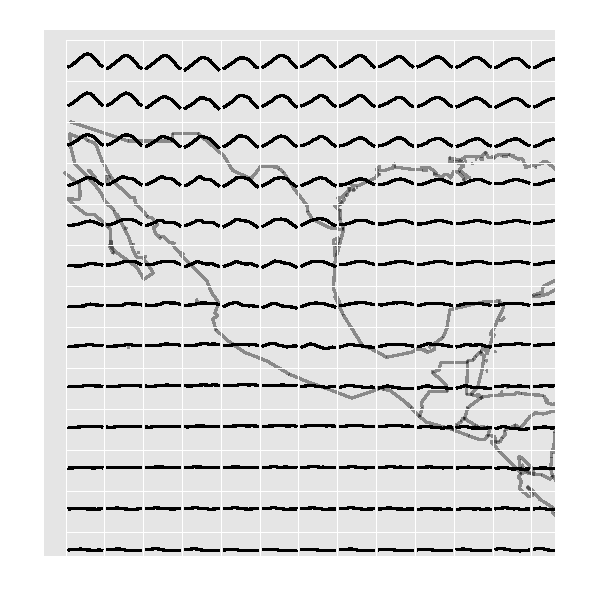
\includegraphics[width=3in]{month-cartesian}
%   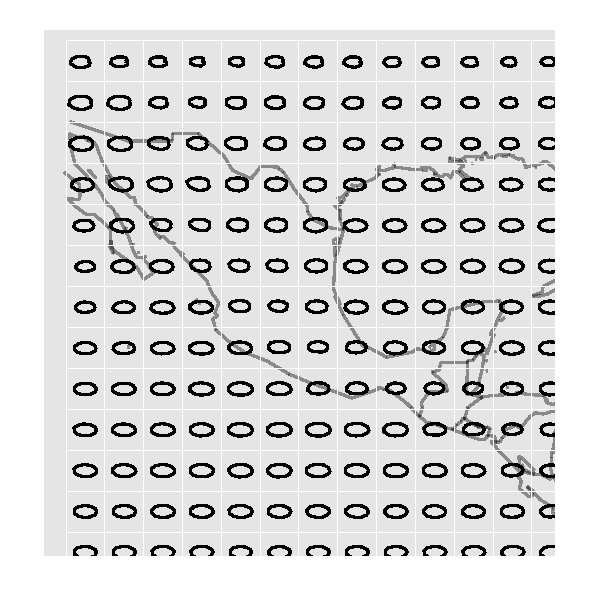
\includegraphics[width=3in]{month-polar}
%     
%   \caption{Monthly averages in (left) Cartesian coordinates and (right) polar coordinates.}
%   
%   \label{fig:cycle}
% \end{figure}

Figure~\ref{fig:templates} gives some small examples of time series with prototypical trends, shown both in Cartesian coordinates and polar coordinates. Differences between linear and nonlinear trend are more apparent in the line-glyphs, and are effectively lost in the star-glyphs, which are most effective in exposing cyclical patterns due to seasonality. Star-glyphs show seasonality as floral cartoons, with peaks forming petals. It is surprising that time series with opposing trends in line-glyphs don't show this symmetry when displayed with star-glyphs. The area of star-glyphs coordinates mainly reflect the average value of a time series, while its shape shows deviations from the average.

\section{Perception}~\label{sec:perception}

All plots facilitate some comparisons and impede others. For a plot to be useful for a particular data analytic task, primary comparisons need to be made the simplest by the display. For climate data, changes in slope, or trend, average value, and variance over time, are the primary tasks. Glyph-maps support these tasks because the pieces of the graphical elements that are needed to make the temporal comparisons are organized, and grouped together.

Glyph-maps allow time trends to be read directly from the plot. Values are mapped to position, one of the easiest properties to perceive, rather than color, which is among the hardest graphical element to parse \citep{cleveland:1984}. Perceiving time trends in faceted heatmaps is much more difficult: not only do you need to read value from color (difficult), you also need to spot the difference (major challenge) between the different maps. From a cognitive perspective these sorts of comparisons can suffer from \emph{change blindness}, often leading to failure to notice the change and not knowing that something changed \citep{healey:2011,busey}. To see this, examine Figures~\ref{fig:nasa-facet} and \ref{fig:nasa-glyph}. The heatmap requires comparing color values across maps to assess temporal change but the glyph-map allows direct reading of the temporal trend at each location, and comparison across spatial neighbors. Conversely, if the purpose is to read spatial trend for one time point the heatmap may be a better choice, because this is a difficult task with the glyph-map. 

% Laying time series out on the spatial grid, the main task expected of the viewer is comparing the temporal patterns from one location to the next. In contrast, in the small multiples used in the facetted colored map, the viewer is expected to compare the patterns in the maps from one year to the next, for corresponding months. (See \citet{carr:1999} for a discussion on perceptual grouping.) That is, compare and contrast maps with facetted colored map, or compare and contrast time series using the glyph-map. 

A possible draw-back of the glyph-map, particularly if linear trend is displayed as an icon, is it may suffer from the Z\"ollner Illusion \citep{Zollner}, which makes straight lines look crooked (Section \ref{sec:large-data} has an example).

Two other factors are critical for accurate perception of change: reference frames and scaling. These are described in the following two sections.

\subsection{Reference frames}~\label{sec:reference}

The structured spatial arrangement of icons in a glyph-map helps to compare the patterns of shape, like slope, intercept, or size, across icons. However, additional clues can make comparisons easier, converting the perceptual task from comparing length to the easier position along a common scale \citep{cleveland:1984}. This is also called a \emph{visual reference grid} \citep{cleveland:1993a}.

Each glyph is small, so there is not enough space for a full set of axes. Instead, minimal reference lines and boxes are incorporated. These need to be minimally perceptible, post-attentive \citep{healey} and de-emphasized, so as not to detract from the data. The reference grid is a box, framing each icon, which represents the spatial grid. The reference line is a horizontal line at mid-range. Both help to read differences in slope and intercept. Slope is read by comparing the position of left and right endpoints on the frame, or by reading the angle between the data line and the reference line. Intercept is read from ``average'' position of the line in the box: is it near the top, or near the bottom? Figure~\ref{fig:ref-basic} demonstrates both guides. Reference elements are drawn in white, so they are minimally perceptible relative to the black data. Average temperatures were calculated for each month, and these were passed to the glyph calculations to produce the glyph-maps.   

% , making it easier to compare the slopprovides for better reading of the intercept. The average value for the temperature anomaly data is not the same across the map: at higher latitudes the temperatures are uniformly higher, but at lower latitudes they are uniformly lower. (**** Can this be right? Would it mean that at these locations the temperatures 1950-2010 are much higher than the reference year temperatures?)

% *** Re-do these figures with zooms in on the GISTEMP data

\begin{figure}[htbp]
  \centering
  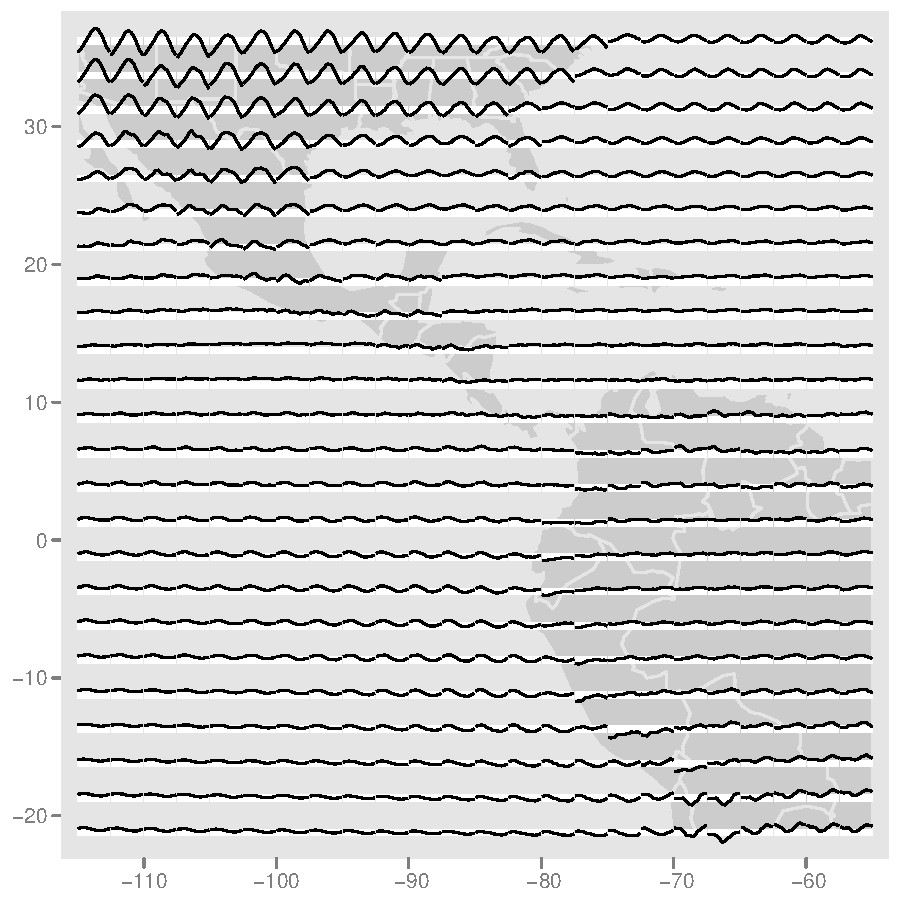
\includegraphics[width=0.5\linewidth]{ref-line}%
  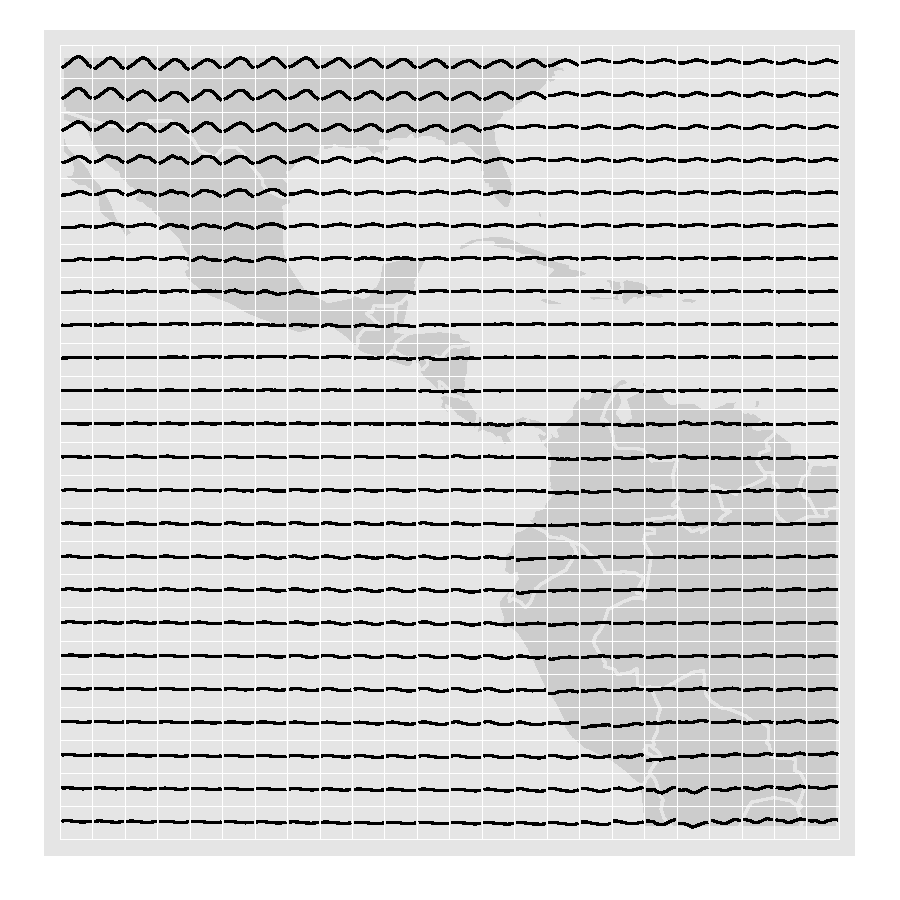
\includegraphics[width=0.5\linewidth]{ref-box}

  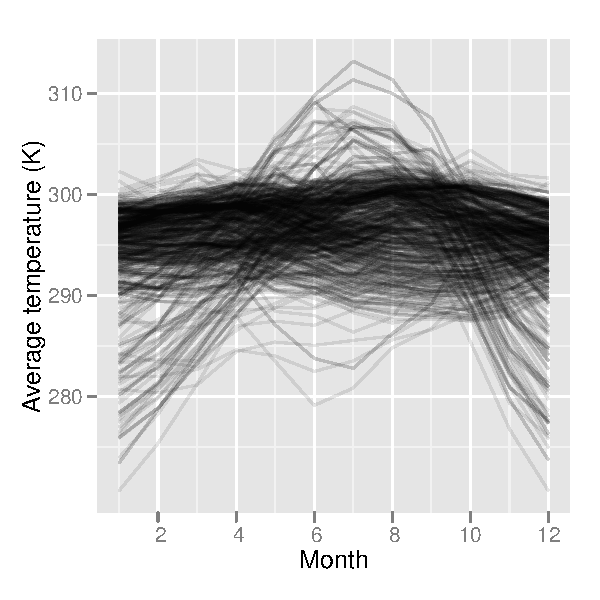
\includegraphics[width=0.33\linewidth]{ref-legend}

  \caption{Glyph-maps of seasonal temperature patterns (averages for each month over all years), using the EXPO data. Adding mid-range reference lines (top left) and grid-cell reference boxes (top right), makes it easier to see differences in glyph position, not just shape. (Bottom) Legend shows temperature values across all locations to aid interpretation.}
  \label{fig:ref-basic}
\end{figure}

For star glyphs the reference frames are also useful and the equivalent of the reference line is a circle (see Figure~\ref{fig:templates}).

%*** Re-visit this next paragraph - its a little too airy-fairy, and the plot with color needs to have the color dampened more. Its way too dominant. This paragraph is too speculative for the paper, so removing it from first draft.

%It's also often useful to display other types of reference information. You are only limited by your imagination (and the capabilities of your graphics software), but two simple ideas are to (1) vary the color or transparency of glyphs or references, or (2) use an additional layer to highlight special points. Figure~\ref{fig:ref-adv} illustrates these ideas to display the month with the highest temperature at each locations. Careful color choice is necessary so that this information is perceptible, but not distracting.

%\begin{figure}[htbp]
%  \centering
%  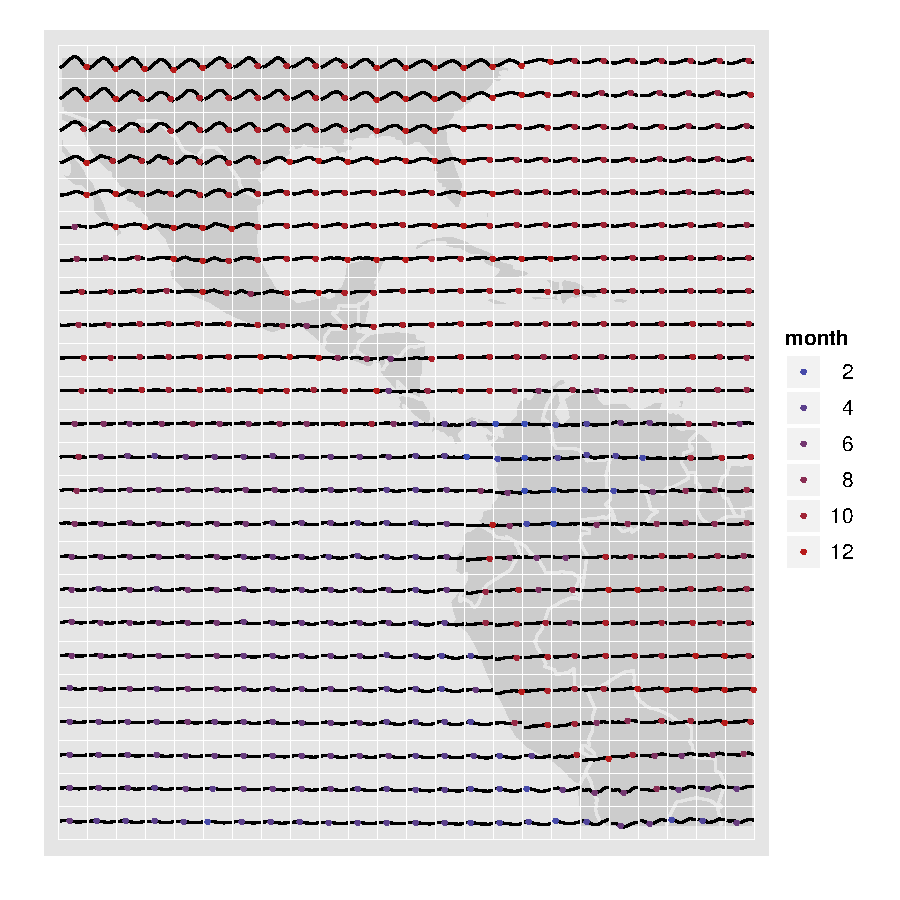
\includegraphics[width=0.5\linewidth]{ref-max-1}%
%  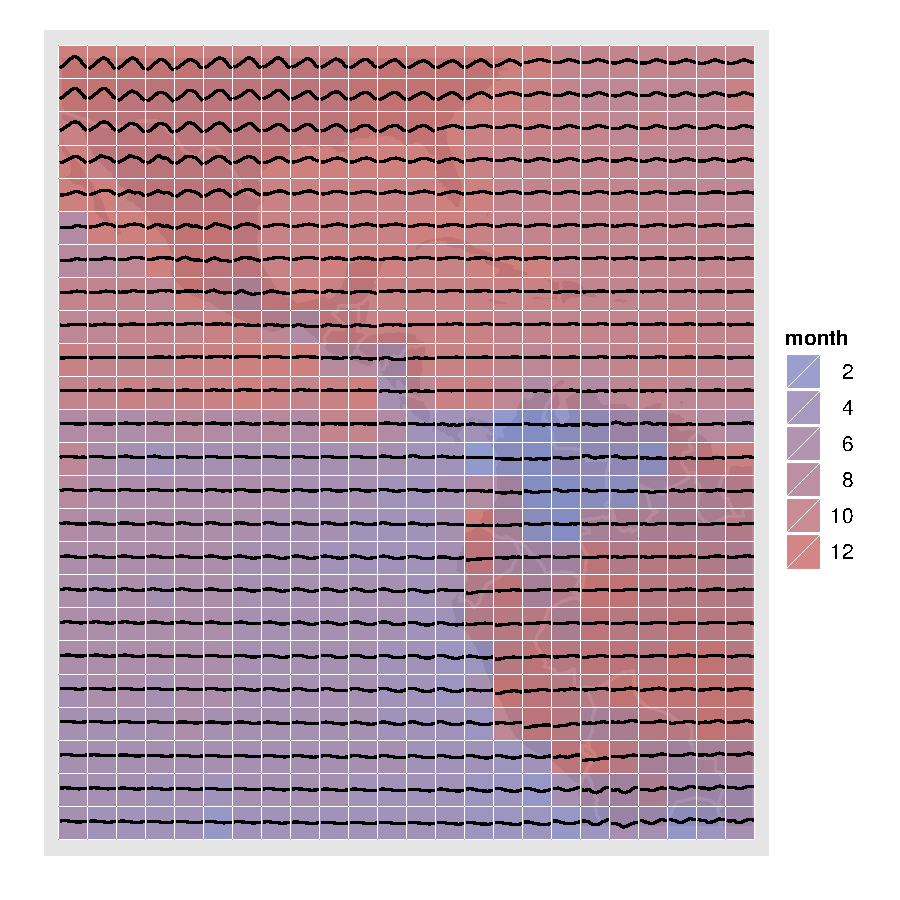
\includegraphics[width=0.5\linewidth]{ref-max-2}
%  \caption{Glyph-maps of seasonal temperature patterns also showing the month with the highest temperature using (left) an additional layer of points and (right) changing the background color of the reference grid.}
%  \label{fig:ref-adv}
%\end{figure}

%A particularly useful summary when to add when displaying model predictions, is some measure of model fit. This makes it easier to avoid over-interpreting predictions from poorly-fitting models.

\subsection{Scaling}~\label{sec:scale}

%*** This section needs to have plots re-done, once we have decided on the key pieces

Different features of the data can be emphasized by varying the scale used with each cell. By default, a global scale is used, so the same position within each cell corresponds to the same value in all locations. This facilitates the comparison of absolute values, and draws attention to plots with large overall variation.

Alternatively, local scale can be used. In local scaling, the values within each location are scaled to range $[0, 1]$ before plot construction. This makes it easier to compare shape (ignoring amplitude), and draws attention to locations with large relative variation. Figure~\ref{fig:scaling} compares global scaling and local scaling for the smoothed temperature data from the EXPO data. (The model is more complicated than the model used previously to de-seasonalize the data. A generalized additive model \citep{wood:2006} with qualitative month and smoothed day terms was fit to the observed data and predicted values were computed for each day of the six year period. Seasonal effects are removed but not overall average or long-term trend.) On the global scale, the El Ni\~no blip in temperature is just visible, along with variation in the average temperature at each location. Local scaling emphasizes the individual shapes: the impact of El Ni\~no can be seen to be over a wider region, linear increases across the Andes, and decreases in the Gulf of Mexico.

\begin{figure}[htbp]
  \centering
  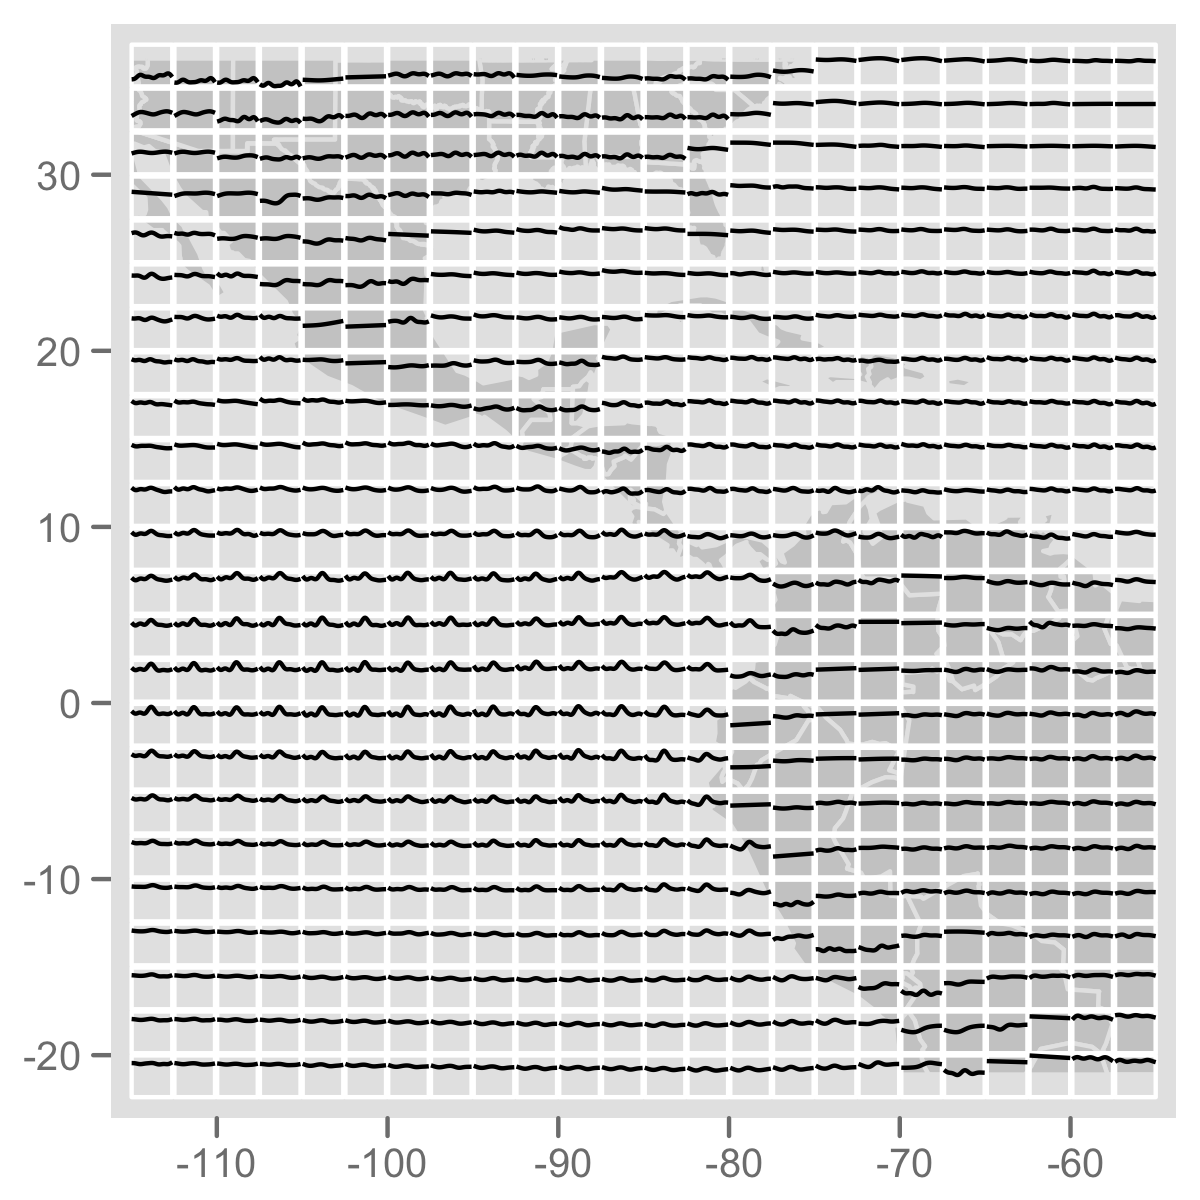
\includegraphics[width=0.5\linewidth]{month-rescale-none}%
  % 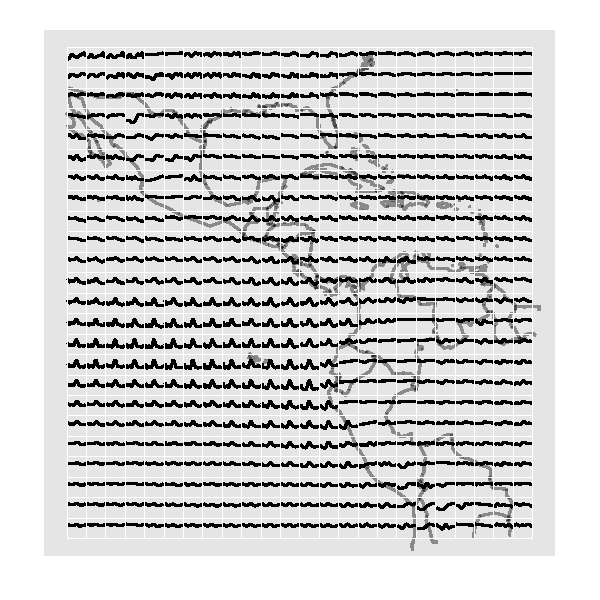
\includegraphics[width=0.5\linewidth]{month-rescale-max}%
  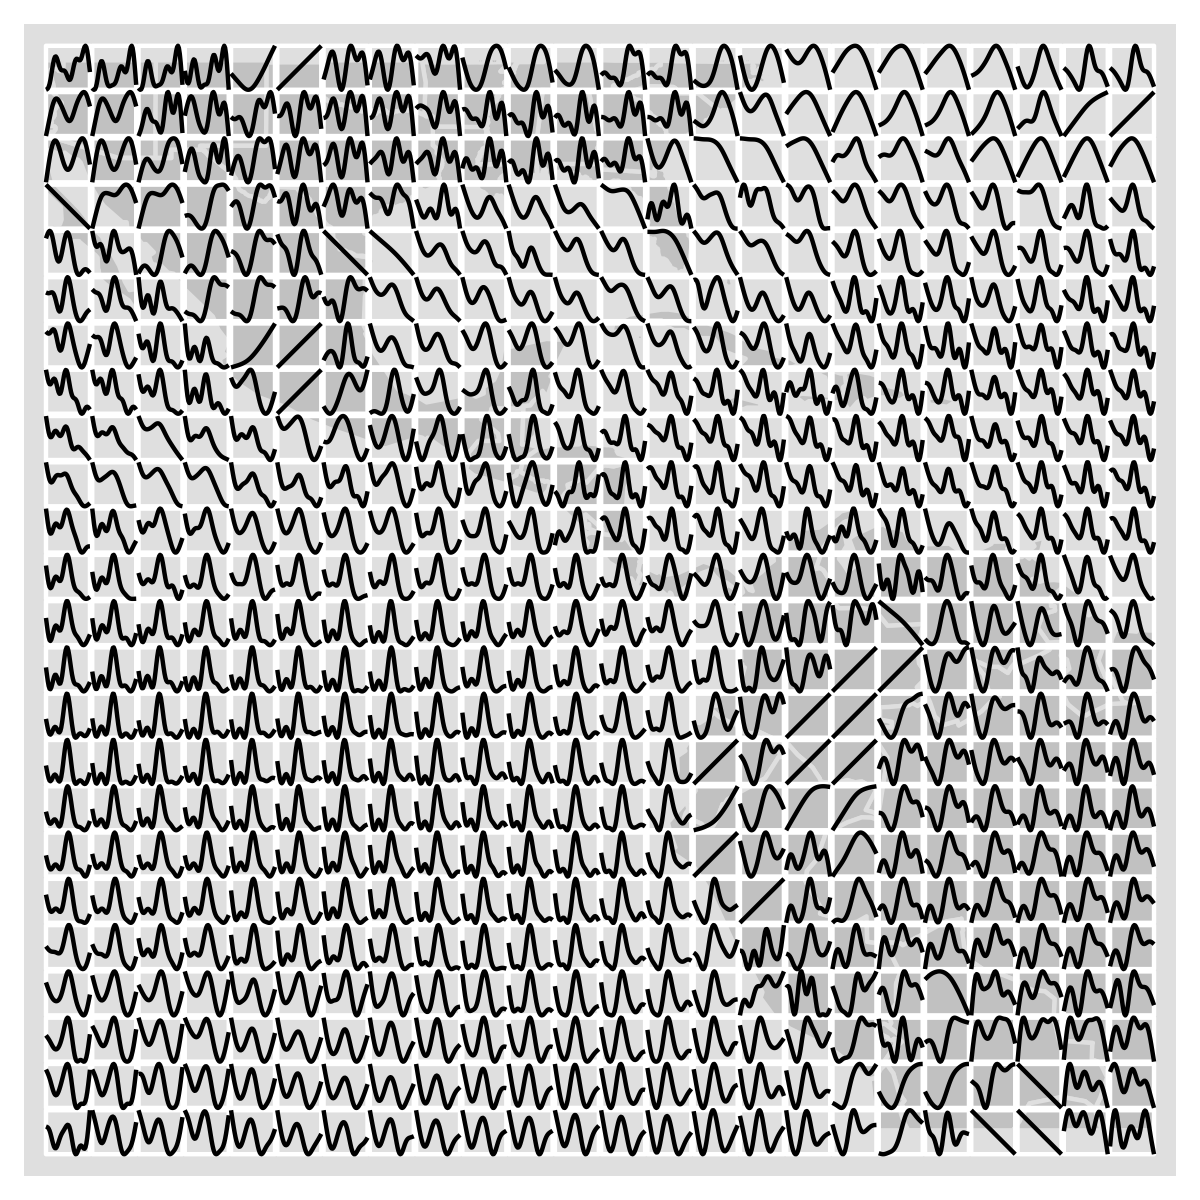
\includegraphics[width=0.5\linewidth]{month-rescale01}

  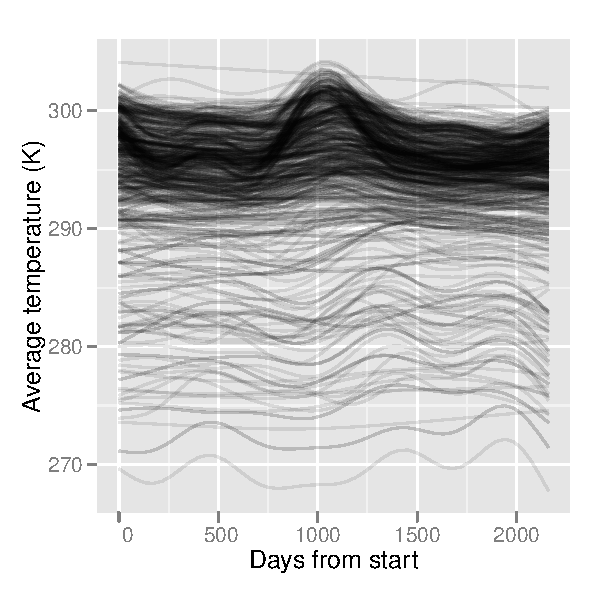
\includegraphics[width=0.33\linewidth]{month-rescale-legend}

  \caption{Glyph-map using predicted daily temperature values from a generalized additive model fit, where seasonality has been extracted: globally scaled (top left), locally scaled (top right). (Bottom) Legend showing ranges of individual glyphs.}
  \label{fig:scaling}
\end{figure}

% 
% \begin{equation}
% y_{st} = \frac{y_{st}-y_{min}}{y_{max}-y_{min}} %\times 2 - 1
% \label{scale1}
% \end{equation}
% 
% \noindent where $y$ is the variable used on the minor axis in equations \ref{coords.eqn}, \ref{coords.polar.eqn}, $y_{min} = \mbox{minimum}\{y_{st}; s=1, \dots S, t=1, ..., T \}, y_{max} = \mbox{maximum}\{y_{st}; s=1, \dots S, t=1, ..., T\}$, $S=$ is the number of spatial locations and $T=$ is the number of time points. In addition, $y_{st}$ may be further scaled by doubling and subtracting 1 to give values between -0.5 and 0.5 for using in equations \ref{coords.eqn}, \ref{coords.polar.eqn}.
% 
% \begin{equation}
% y_{st} = \frac{y_{st}-y_{s,min}}{y_{s,max}-y_{s,min}} %\times 2 - 1
% \label{scale2}
% \end{equation}
% 
% \noindent where $y_{s, min} = \mbox{minimum}\{y_{st}; t=1, ..., T \}, y_{s,max} = \mbox{maximum}\{y_{st}; t=1, ..., T\}$. 

Other types of shifting and scaling can be useful:

\begin{itemize} \itemsep 0in

  \item The mean and standard deviation (or robust equivalents) could be used
  to standardize values to common moments.
  
   \item Scaling to maximum 1 (but leaving the minimum unchanged) can help
  emphasis the relative shape, but not distort the range as much as rescaling
  to range $[0, 1]$.

  \item Shifting the values at each location to have mean zero places more
  focus on the trend. This is particularly important for the star glyphs,
  where differences in the average value lead to unintuitive patterns in the
  resulting glyphs.

\end{itemize}

Note that the use of local scales needs to be clearly marked. The viewer must realize that the scale is not relative and that big patterns in some locations might be just tiny effects. To indicate this on the locally scaled data plots, one can use an additional aesthetic, like color, to encode the range of original scale. This is illustrated in Figure~\ref{fig:scaling-col}. In the encoding, emphasis is placed on the locations with larger range, stronger effects: the line intensity is stronger (left plot), and the background is lightened to provide greater contrast (right plot) drawing the eye to these regions. 

\begin{figure}[htbp]
 \centering
 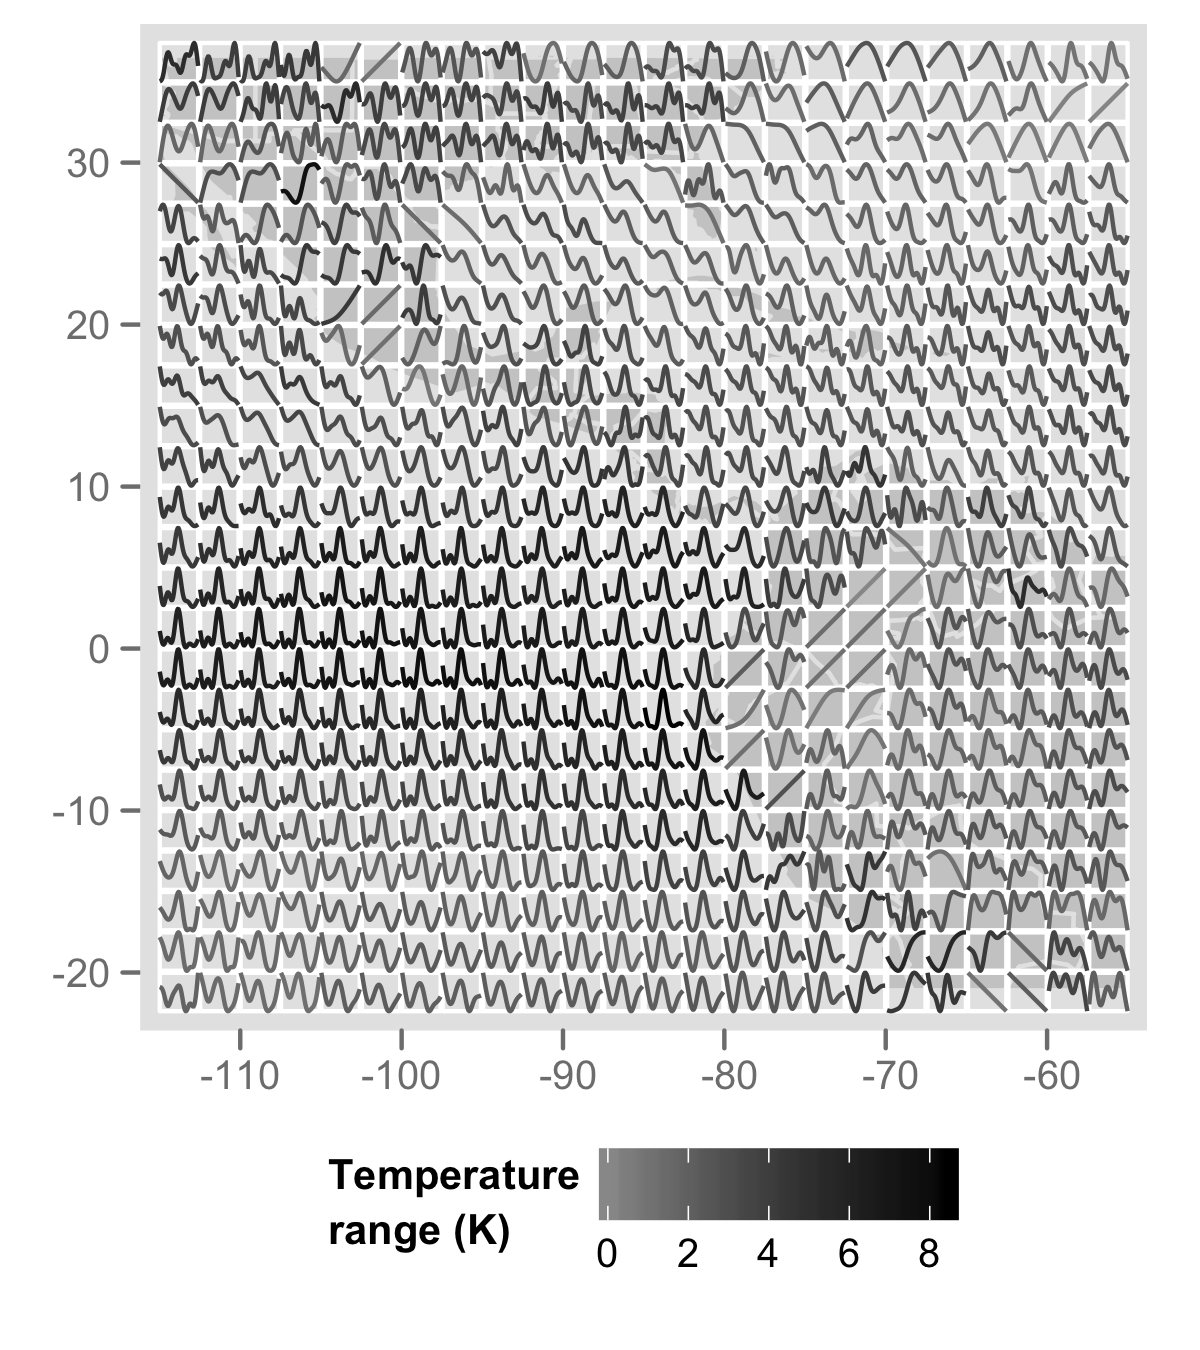
\includegraphics[width=0.5\linewidth]{month-rescale01-col}%
 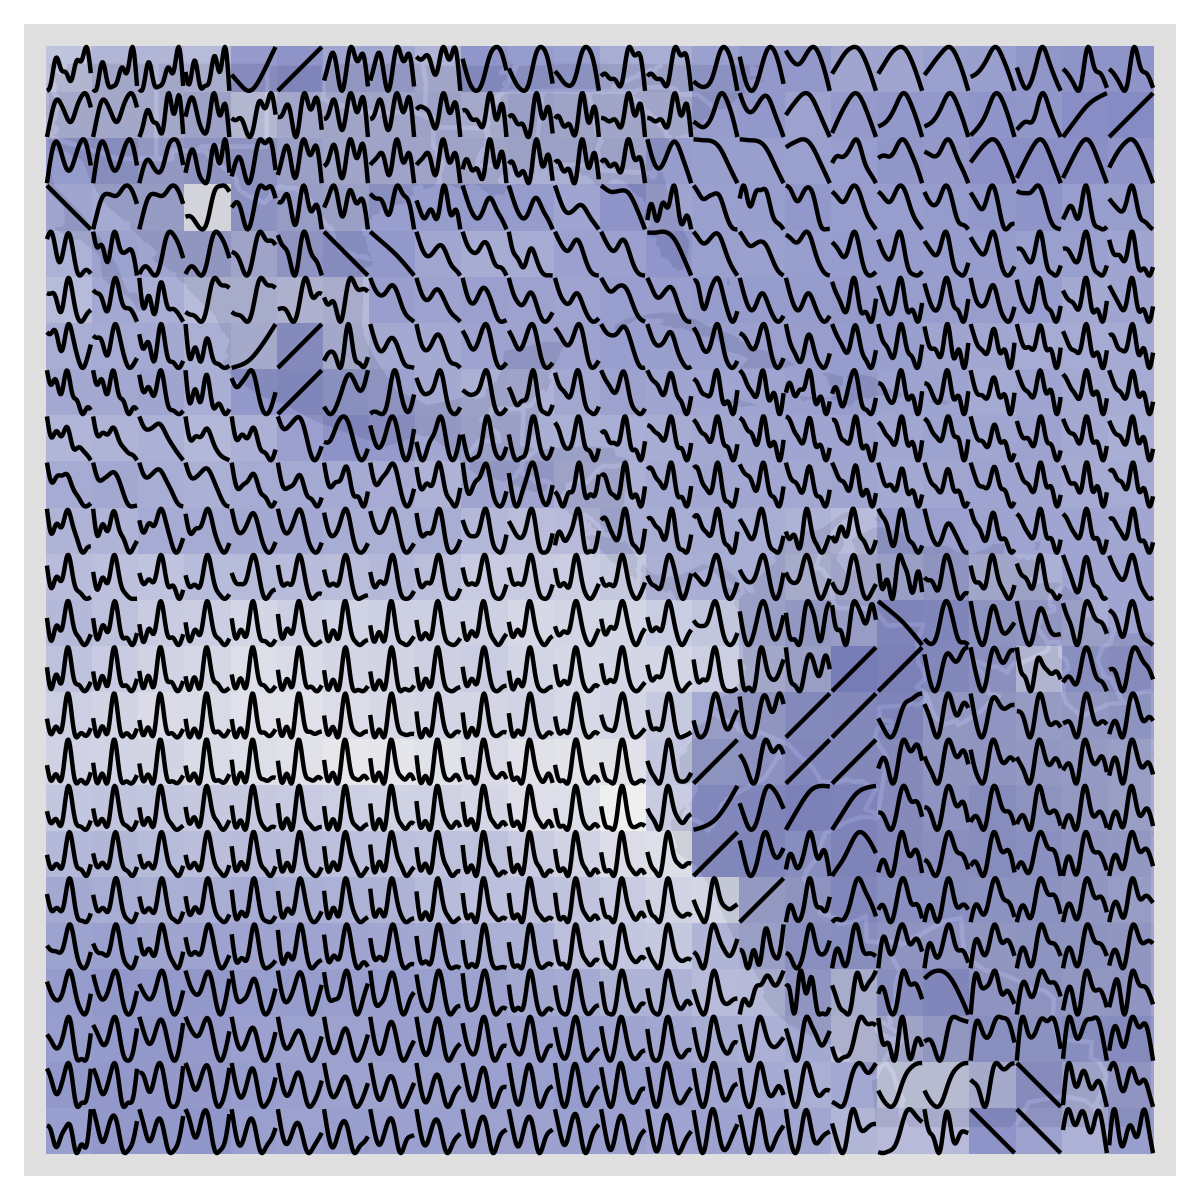
\includegraphics[width=0.5\linewidth]{month-rescale01-fill}
 \caption{Adding intensity and color to scaled plots. Here each location has been scaled to range $[0, 1]$ and color mapped to the range of the original predictions. (Left) Range mapped to intensity (grey scale) of the line: pale locations have smaller range, smaller effect, than darker locations, stronger effect. (Right) Range mapped to fill color of grid box: blue boxes have smaller ranges, and light boxes have larger effects. Shapes at all locations are visible, but attention is drawn to locations with lighter backgrounds, larger ranges, because of the higher contrast.}
 \label{fig:scaling-col}
\end{figure}

One more important point: if a model summary is displayed in the glyph-map, as discussed in the following section, it may be important to force the scale to that of the original data. The range of predicted values is typically smaller than the raw data, so angles of slopes is increased, giving an inaccurate sense of a stronger effect.  

% Displaying the predicted values in the absence of the raw data scale typically increases magnitude because the variation is much lower.

\section{Large data and models}
\label{sec:large-data}

Climate data is usually large: many locations in space, and many points in time, which can make it arduous to work with computationally. The glyph-map calculations are as efficient as possible computationally, being linear in the number of spatial locations. It is possible that the calculations could also be paralellized for massive amounts of climate model data. Visualizing large data also hits a perceptual boundary.  There is a limit to the resolution of human visual system \citep{Kr12} which will prevent perfect perception of large spatial domains or seasonality of many years of data. Exploring large data requires reducing it to a resolution that can be reasonably absorbed visually.


Figure~\ref{fig:gistemp-pred} shows the glyph-map for the GISTEMP dataset, which is more realistically sized than the EXPO data. Glyphs at each location represent temperature from 1880--2011, starting with Jan 1880 at 12 o'clock and proceeding clockwise to 2011 at 11:59. The most important feature to notice is the pattern of missing values. Most glyphs do not complete the full circle, typically missing points between 12 and 1, suggesting missing values in the earliest part of the data. Another important feature is variability, shown by the thickness of the circle. Some locations, particularly in the north western mountain region, have large variations in temperature. 

\begin{figure}[htbp]
  \centering
  %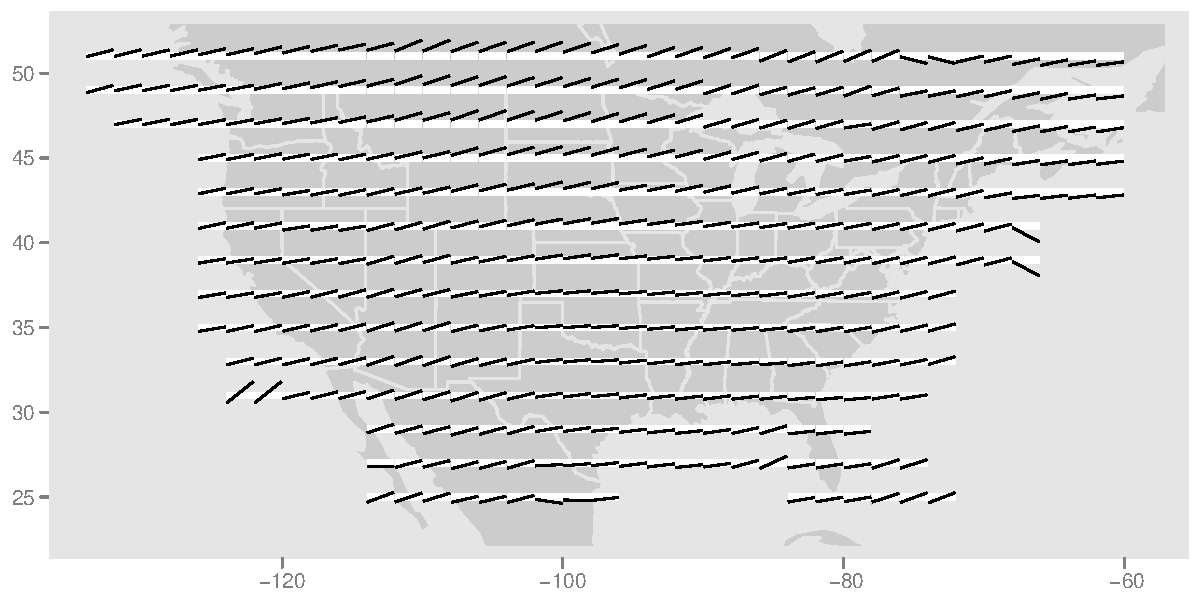
\includegraphics[width=1\linewidth]{gistemp-pred}%

  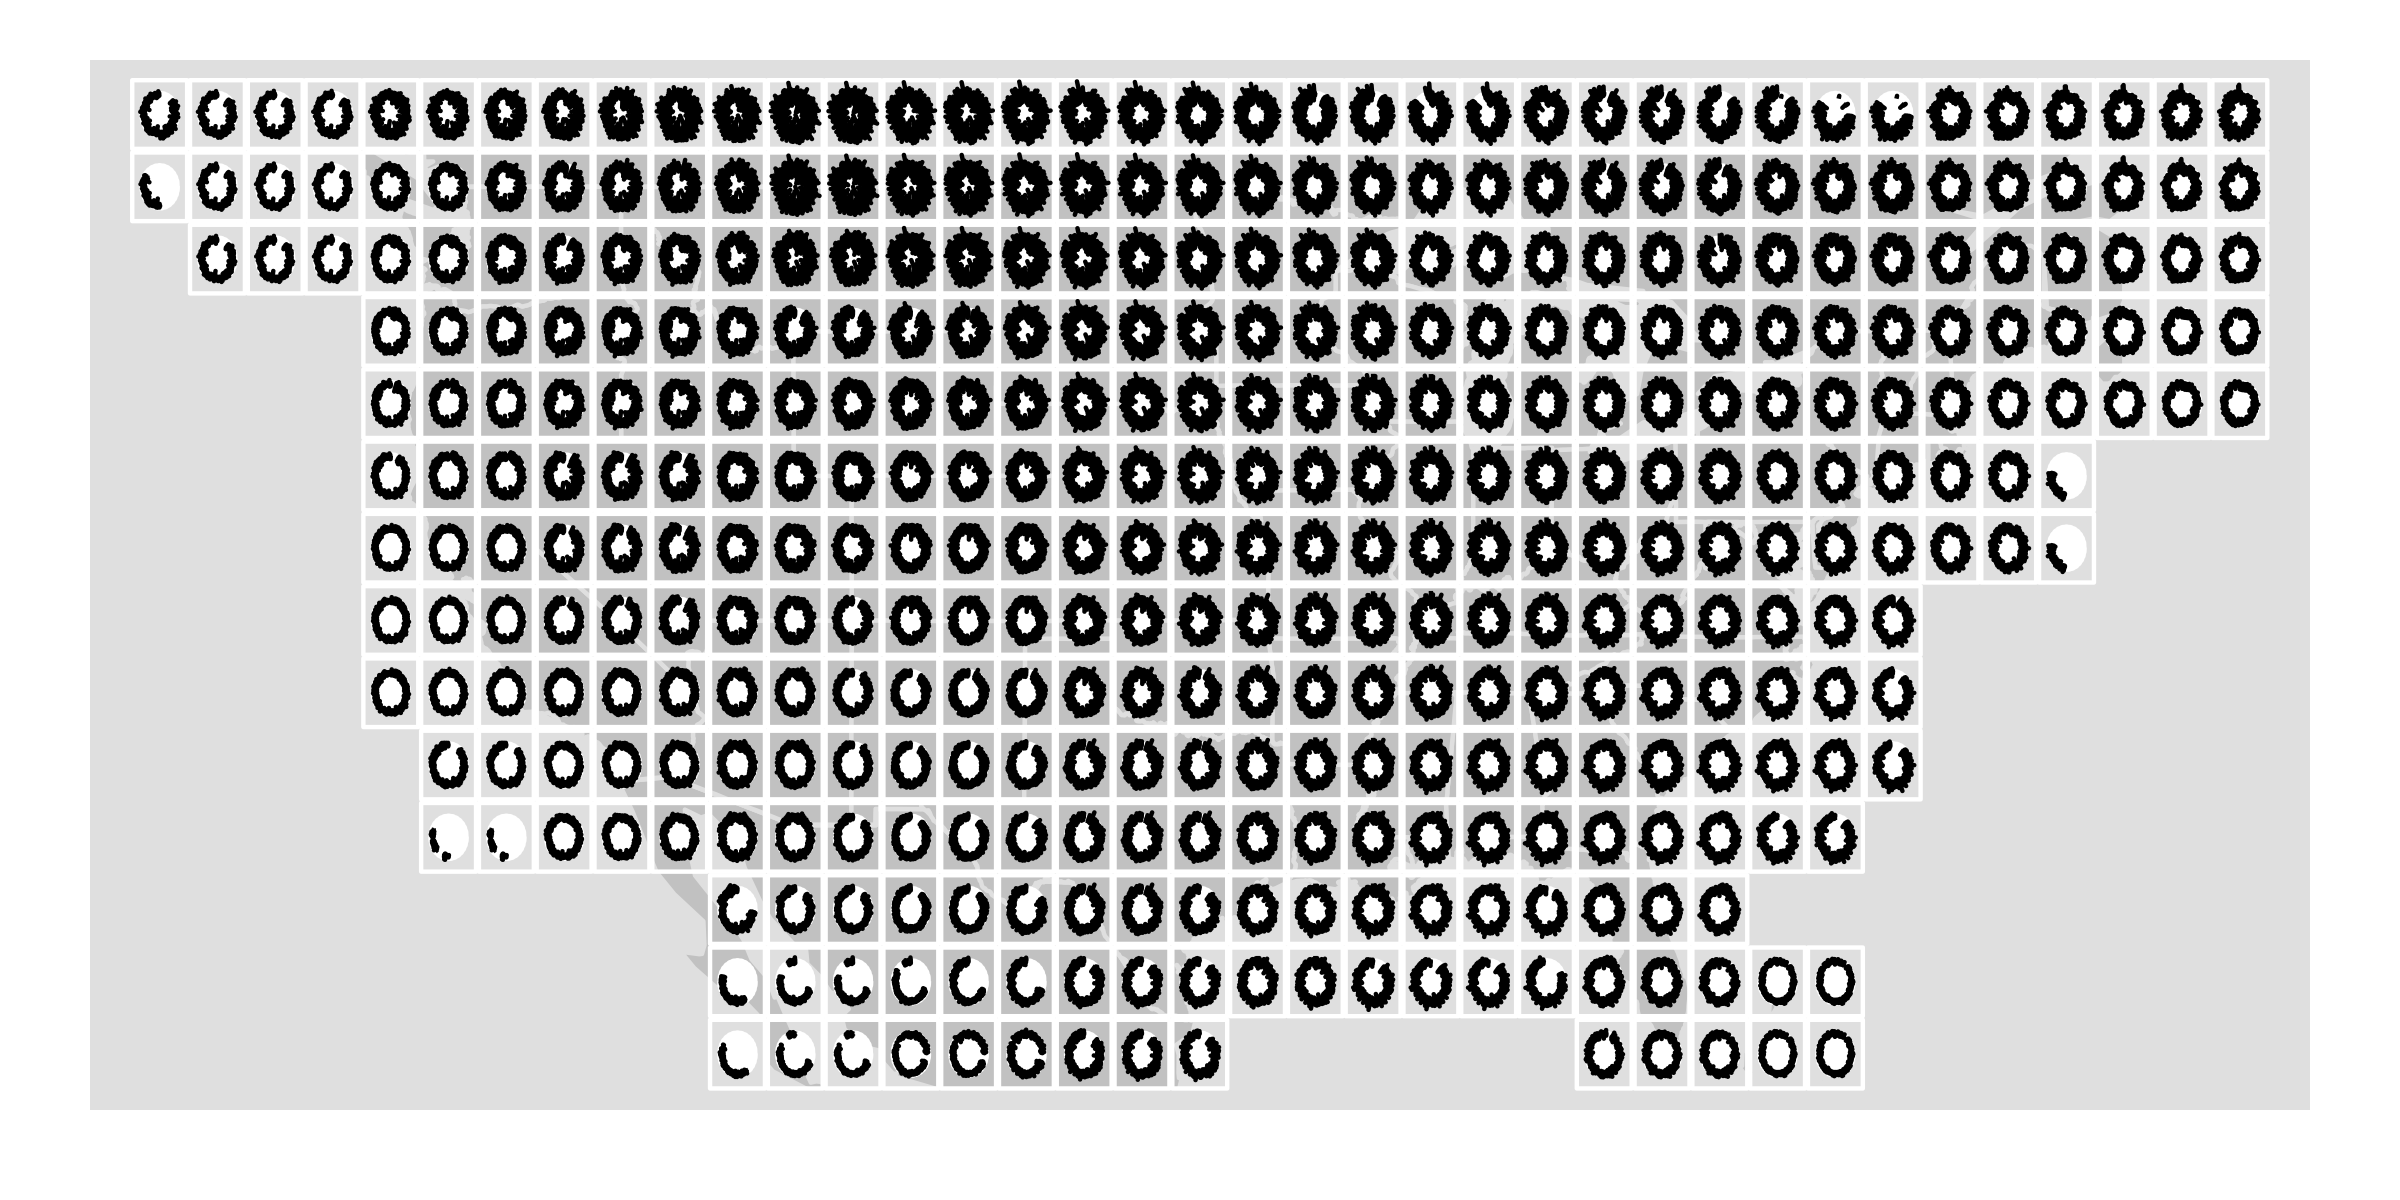
\includegraphics[width=1\linewidth]{gistemp-polar-raw}

  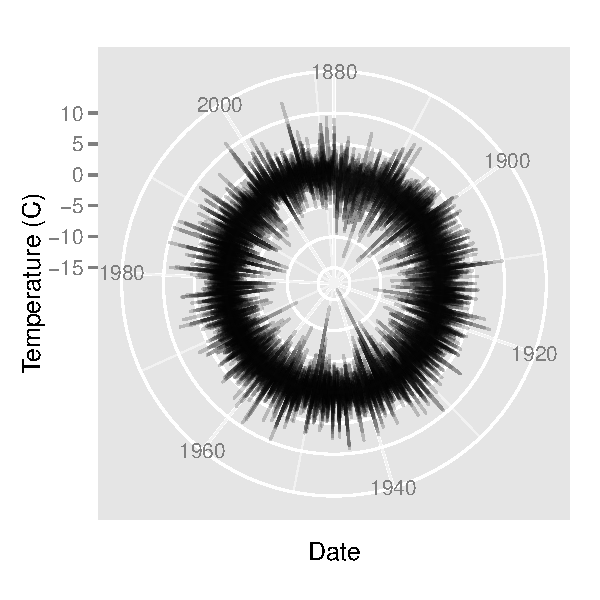
\includegraphics[width=0.33\linewidth]{gistemp-polar-legend}

  \caption{(Top) Glyph-map of raw temperature anomaly data (GISTEMP), from 1880-2011. Gaps in the full circle indicate missing values, and thickness of the circle indicates more variability in the measurements.  (Bottom) Legend showing temperature and temporal ranges of individual glyphs.}
  \label{fig:gistemp-raw}
\end{figure}

The raw data shows us missing values and gives some sense of variability, but gives no information about long-term trend. Statistical models are useful for pre-processing climate data, to decompose data into long-term trend, seasonal effects and error, which is vital for making the problem both computationally and visually tractable. Trend is examined by fitting a linear model to each location and displaying predicted values in Figure~\ref{fig:gistemp-pred}. This plot shows long-term (de-seasonalized) temperature trend for 1950--2010 (the limited time period used due to missing data). Most locations have increasing temperature over this time period. Only a few locations show a decline, and these few locations tend to be different from their neighbors, and on the edge of the data collection region, indicating that there might be isolated data problems. The rate of increase differs across regions: steeper inclines in the north and western mountain regions and across the Great Lakes, and flatter inclines in the southeastern USA.

\begin{figure}[htbp]
  \centering
  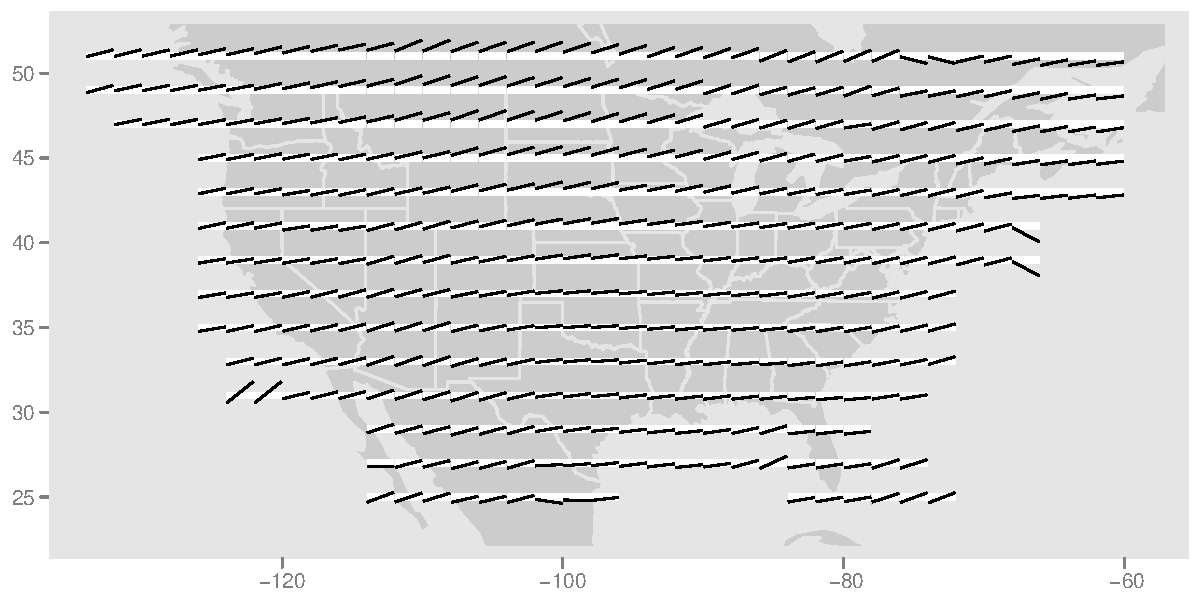
\includegraphics[width=1\linewidth]{gistemp-pred}

  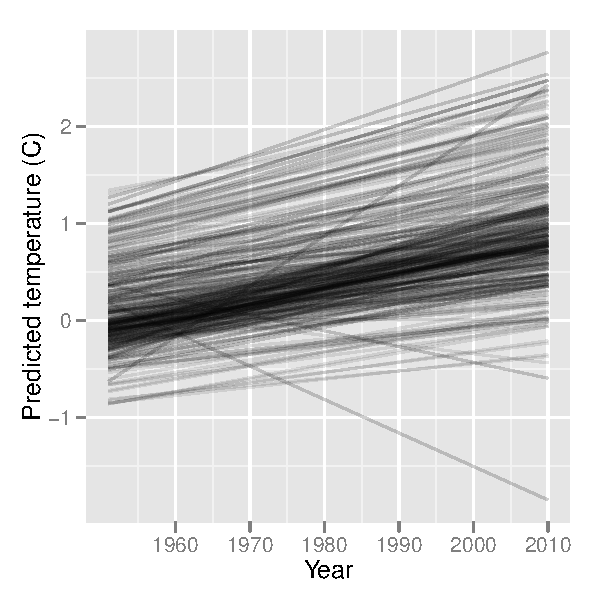
\includegraphics[width=0.33\linewidth]{gistemp-pred-legend}
  %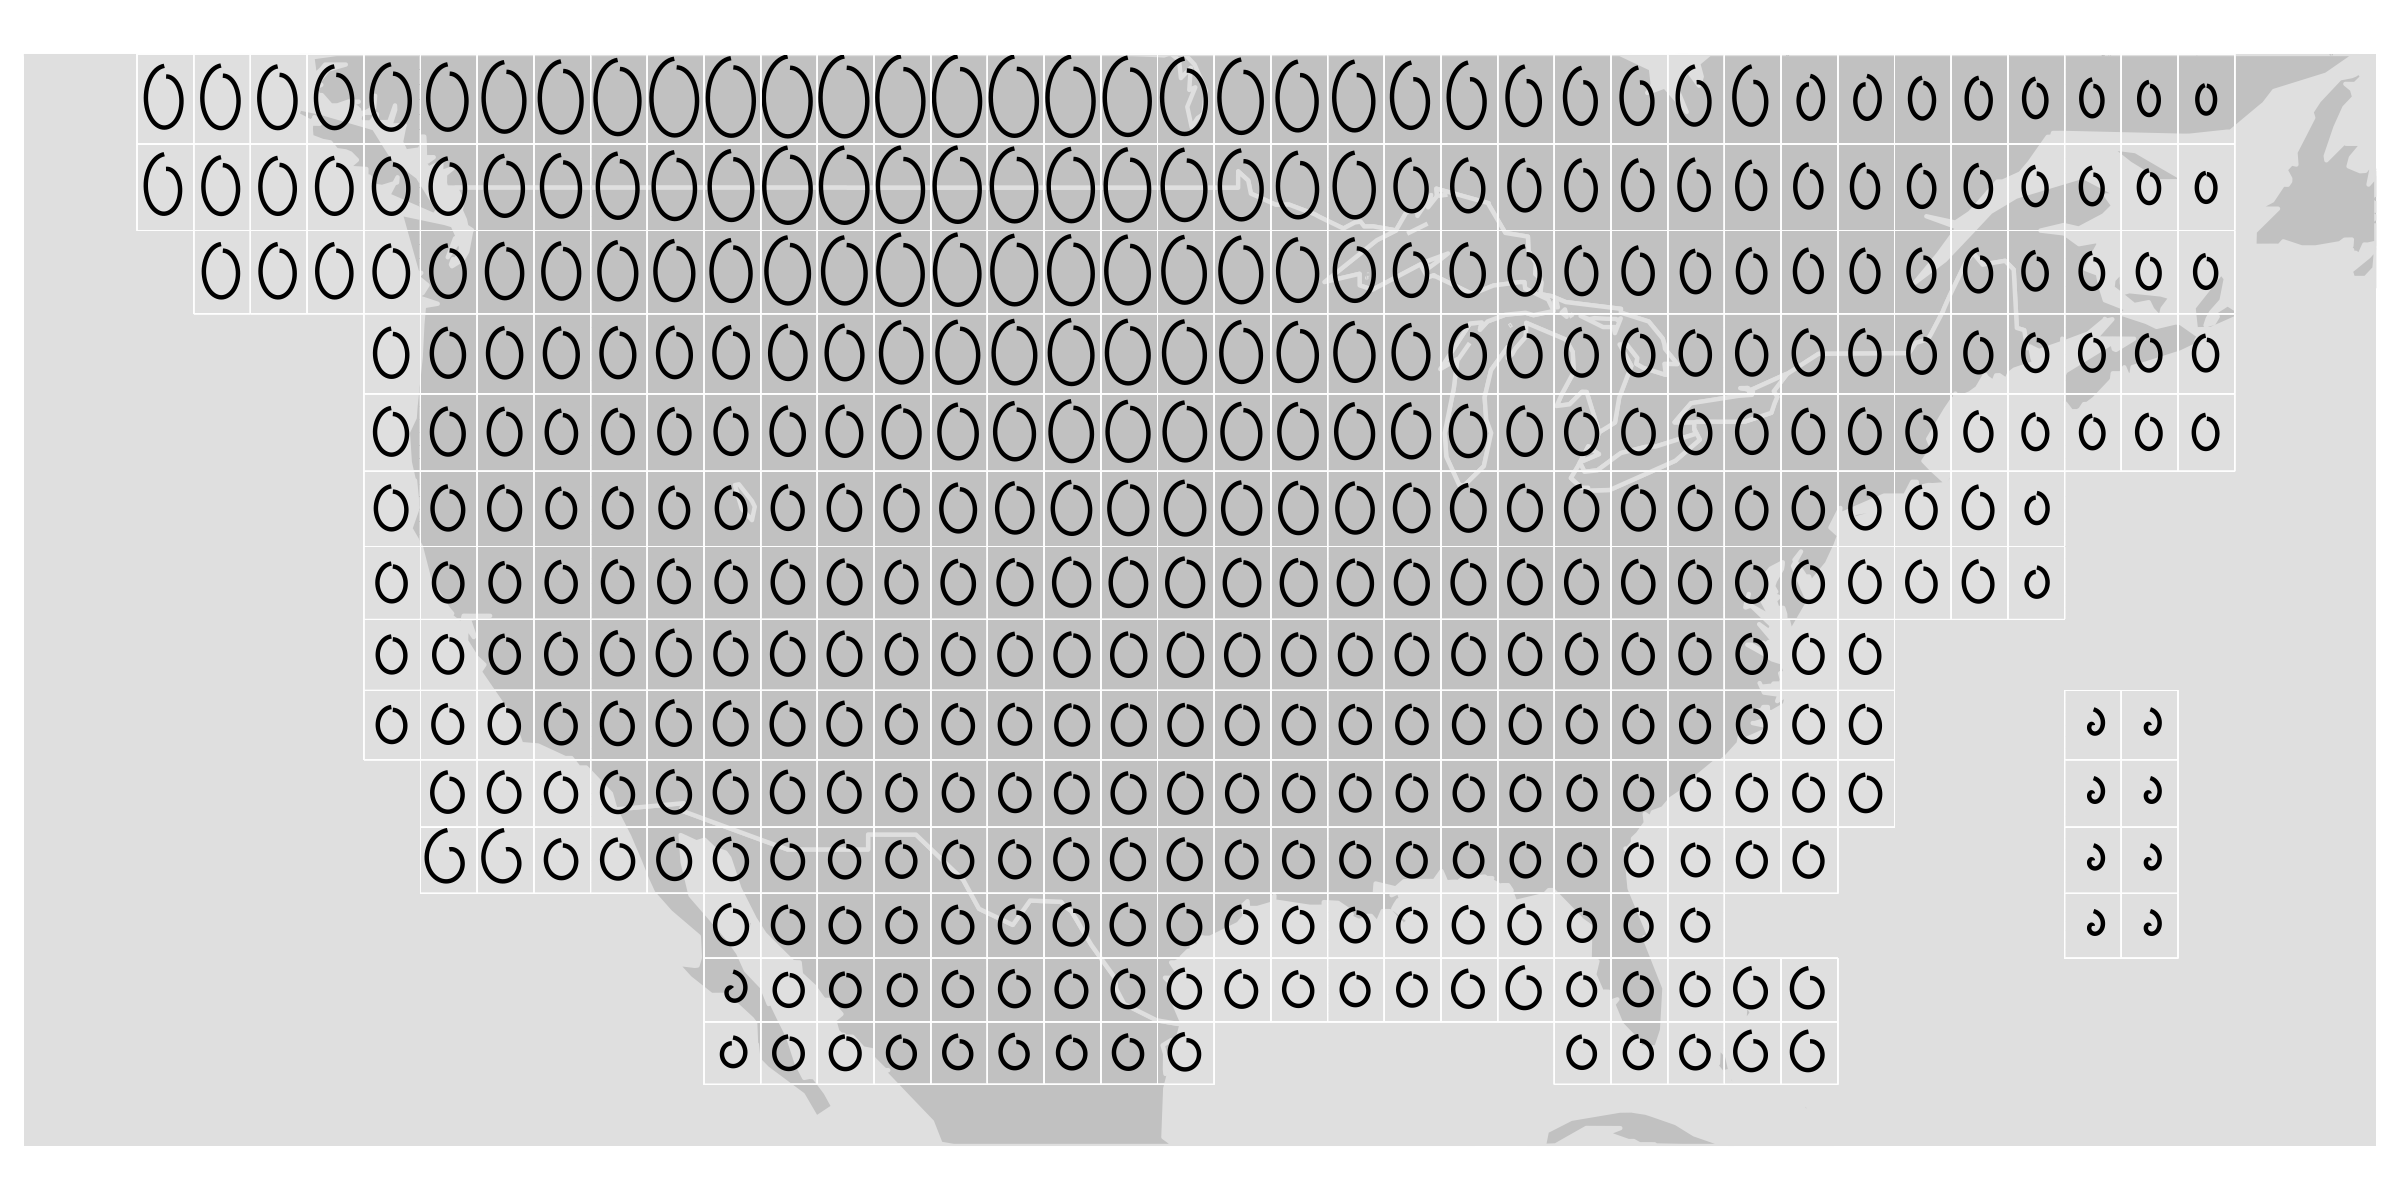
\includegraphics[width=1\linewidth]{gistemp-polar-pred}

  \caption{(Top) Glyph-map of predicted temperature anomaly data
    (GISTEMP), on reduced range temperature 1950-2010. Increasing
    trends can be seen over most of the USA, with varying degrees of
    increase. Some isolated locations exhibit steep declines, and
    inclines, perhaps indicative of some isolated data problems. Note
    that, the reference lines are straight, but they look curved
    because of the Z\"ollner optical illusion. (Bottom) Legend showing
    temperature and temporal ranges of individual glyphs.}
  \label{fig:gistemp-pred}
\end{figure}

%The most seasonality occurs in north American. Some seasonal effects can also be seen in the Caribbean and in south American locations. Around the equator the temperatures are relatively warm for all seasons. Instead of radially displaying the temperature a glyph can be a regular time series, time displayed horizontally and temperature vertically (right plot). The structure perceived is different with this change in glyph type: locations at the equator have flat series, on land more varied temperatures. 

% \section{What to plot: raw data, trend lines, residuals,  seasonal}
% 
% A generalized additive model \citep{wood:2006} with a seasonal term and a long-term smooth term can be useful. This is revealing for smooth models of surface temperature, shown in Figure~\ref{fig:scaling}. Each location is modeled using a generalized additive model \citep{wood:2006} with a seasonal term and a long-term smooth term. The three plots in the figure show the long-term smooth term. 
% 
% %Because some locations are uniformly warmer than others, the impact of
% %changes across time are diminished. In the center plot, each location is
% %scaled by dividing out the maximum, and on the right, each location is scaled
% %to range $[0, 1]$. These emphasize individual changes but lose the ability to
% %make global comparisons, and need caution when interpreting - a small
% %absolute change gets blown up into a large relative change.
% 
% *** Need three plots here: trend, seasonality and residuals, shall we do this with NASA ozone data or stick to temperature?
% 
% Issues of scale relative to modeling. Switching from the data to model summaries brings new scaling issues. Often the scale of the raw data is ignored when the model is plotted, one usually shows just the line showing the trend, in the range of the trend. This has the effect of exaggerating the significance of the model. Scaling the trend lines relative to the range of the data may be useful sometimes.

\section{Non-gridded data}~\label{sec:irregular}

Regularly gridded spatial data helps with the perception of structure, because it helps to provide the reference frames upon which to make comparisons among the icons. When spatial locations are not on a regular grid, some difficulties arise. In this situation it is not clear what the scale of icons should be, there is no regular spacing. Some locations may be close to each other which would generate icons that overlap. 

\subsection{Non-rectangular grids}

Glyph-maps work best when displayed in the coordinate system in which the grid is rectangular and regular.  For example, the GISTEMP grid is 2$^o$ square and is displayed treating longitude and latitude as Cartesian coordinates in Figure \ref{fig:gistemp-pred}.  For regularly gridded data, this results in icons that are rectangles of equal size.  It is often preferable to display maps as a projection of the geographical coordinates which preserves a property of interest, area for example. When a projection is desired a choice needs to be made between applying the projection to the completed glyph-map, or to just the spatial locations.  When the completed glyph-map is projected the icons are no longer rectangles of the same size but they do retain their space filling property.  When applying a projection to the spatial locations and then constructing a glyph-map, the grid becomes irregular. 

\subsection{Irregular locations}
Figure \ref{fig:irregular} shows linear trends for monthly average surface temperature at stations in the USHCN data.  It illustrates three challenges in working with irregular locations: there is no natural choice for icon size, icons can potentially overlap, and comparisons rely more heavily on the reference guides.  The icon sizes were chosen manually for these two plots, although the icons are displayed at about the same size, they correspond to 1$^o$ and 0.5$^o$ square respectively in the geographical coordinates. 
\begin{figure}[htbp]
  \centering
  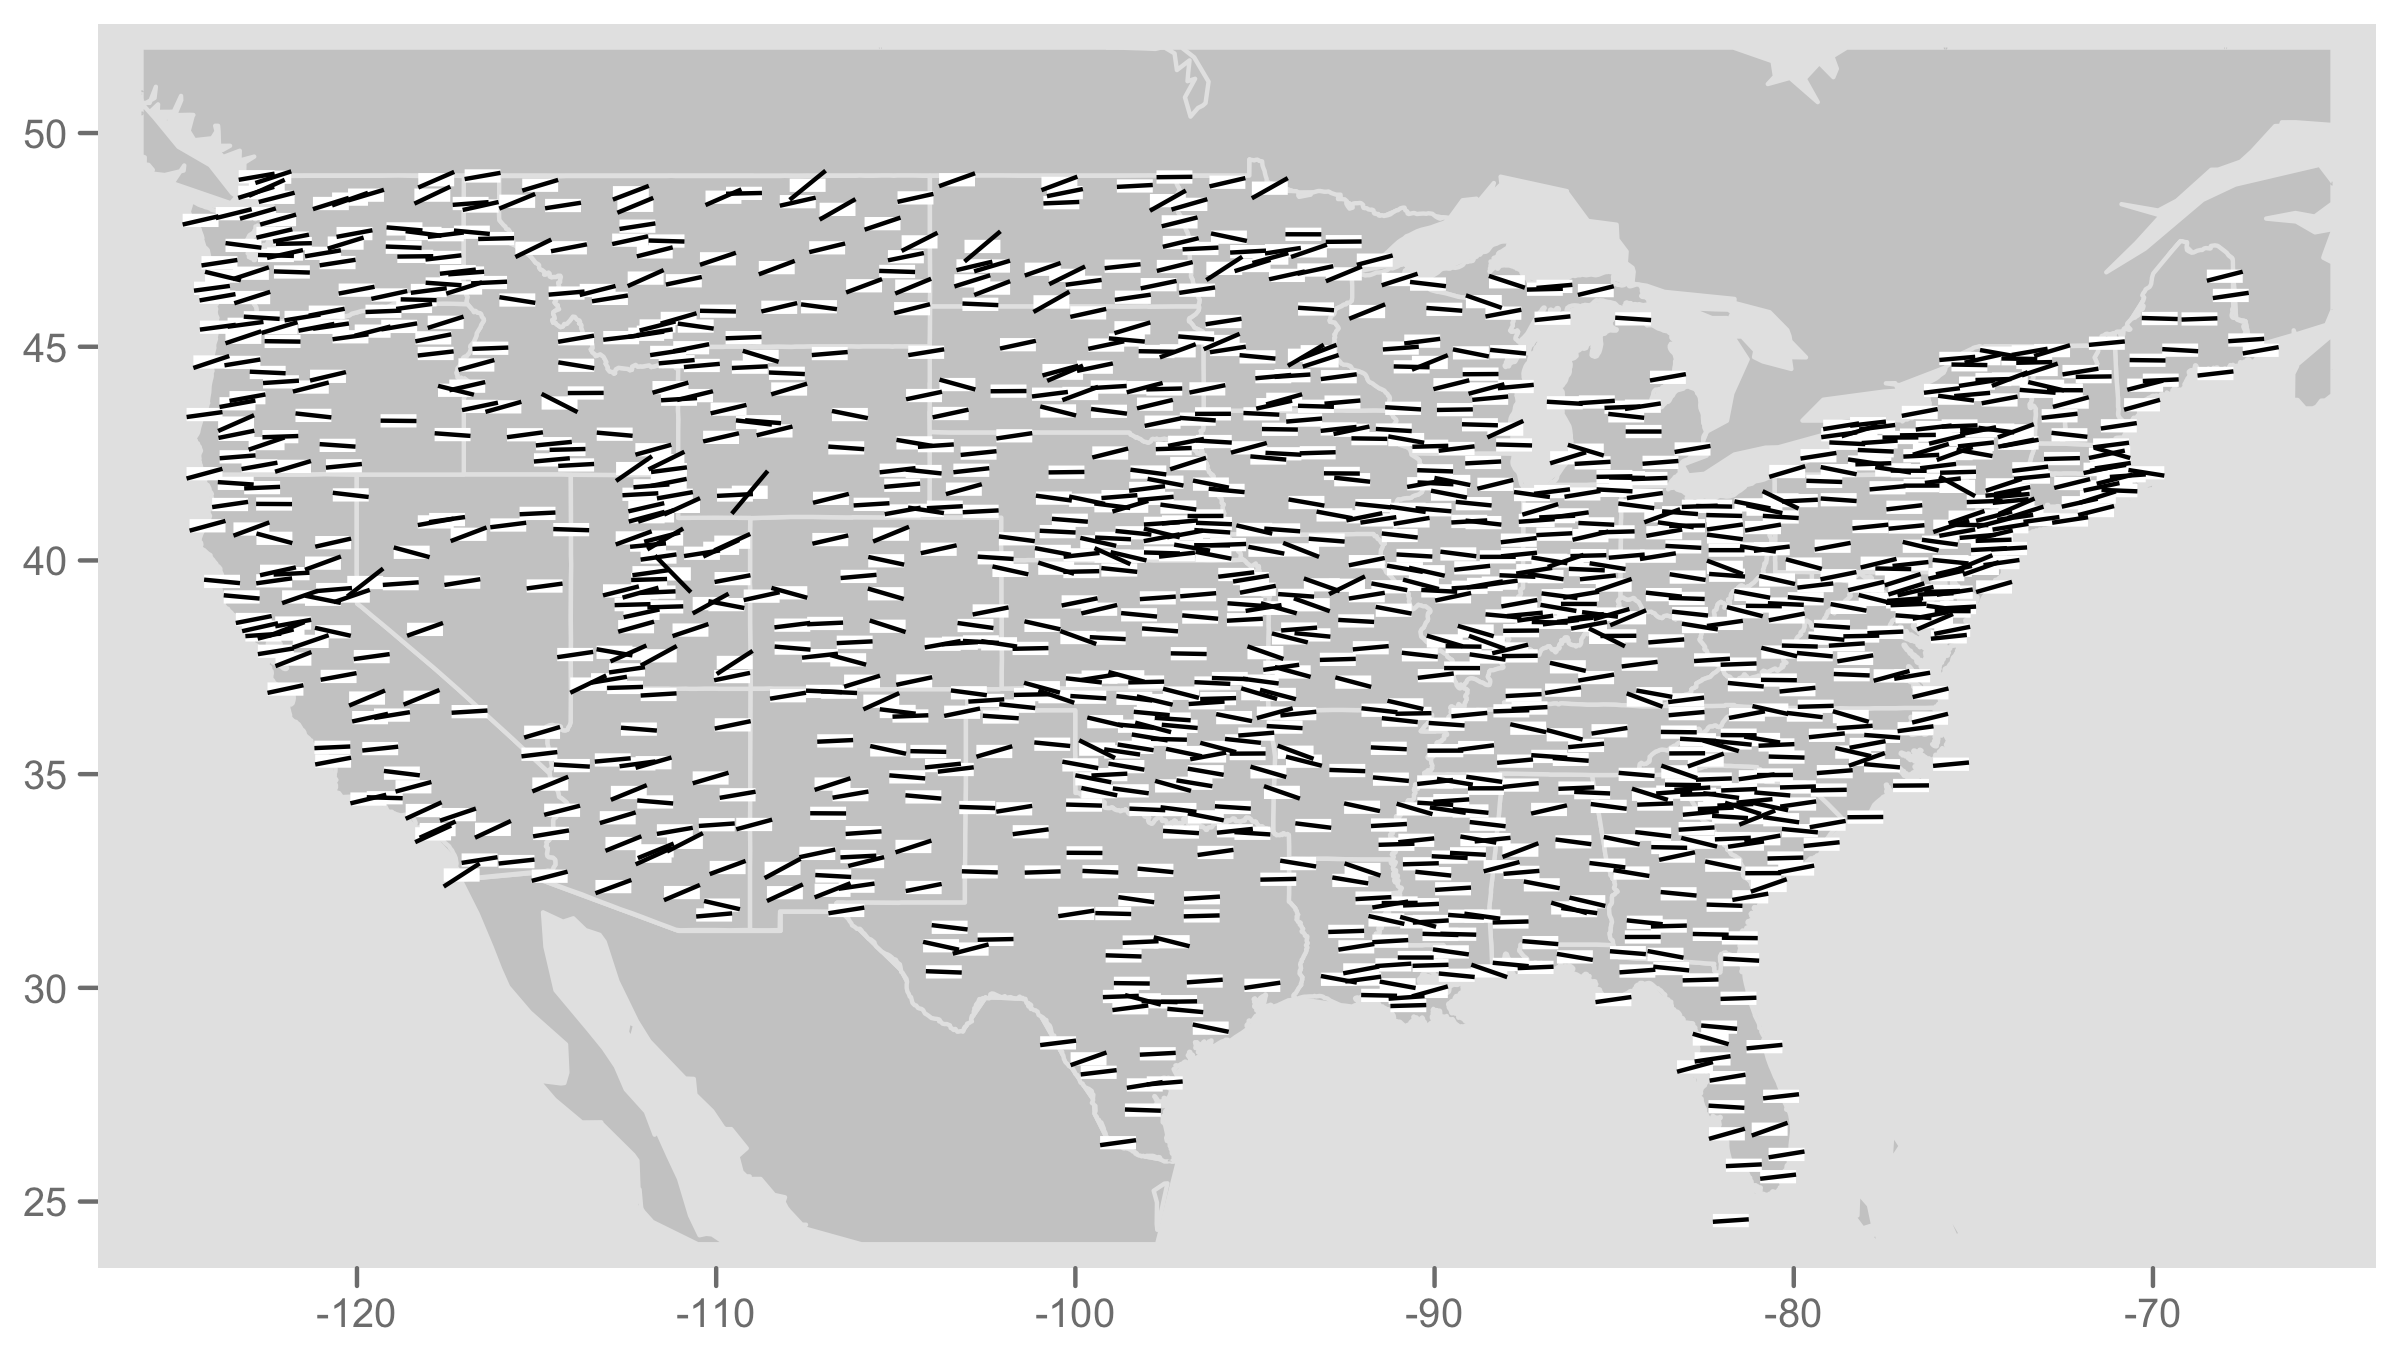
\includegraphics[width=1\linewidth]{usa-lin-overlap}%

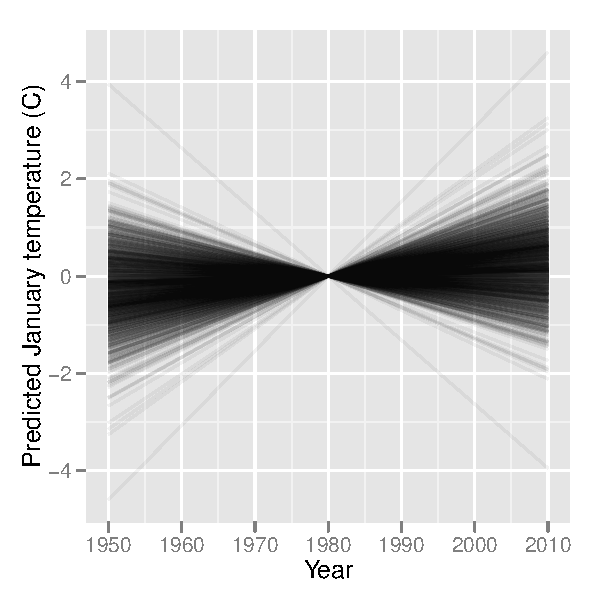
\includegraphics[width=0.33\linewidth]{usa-lin-legend}
  %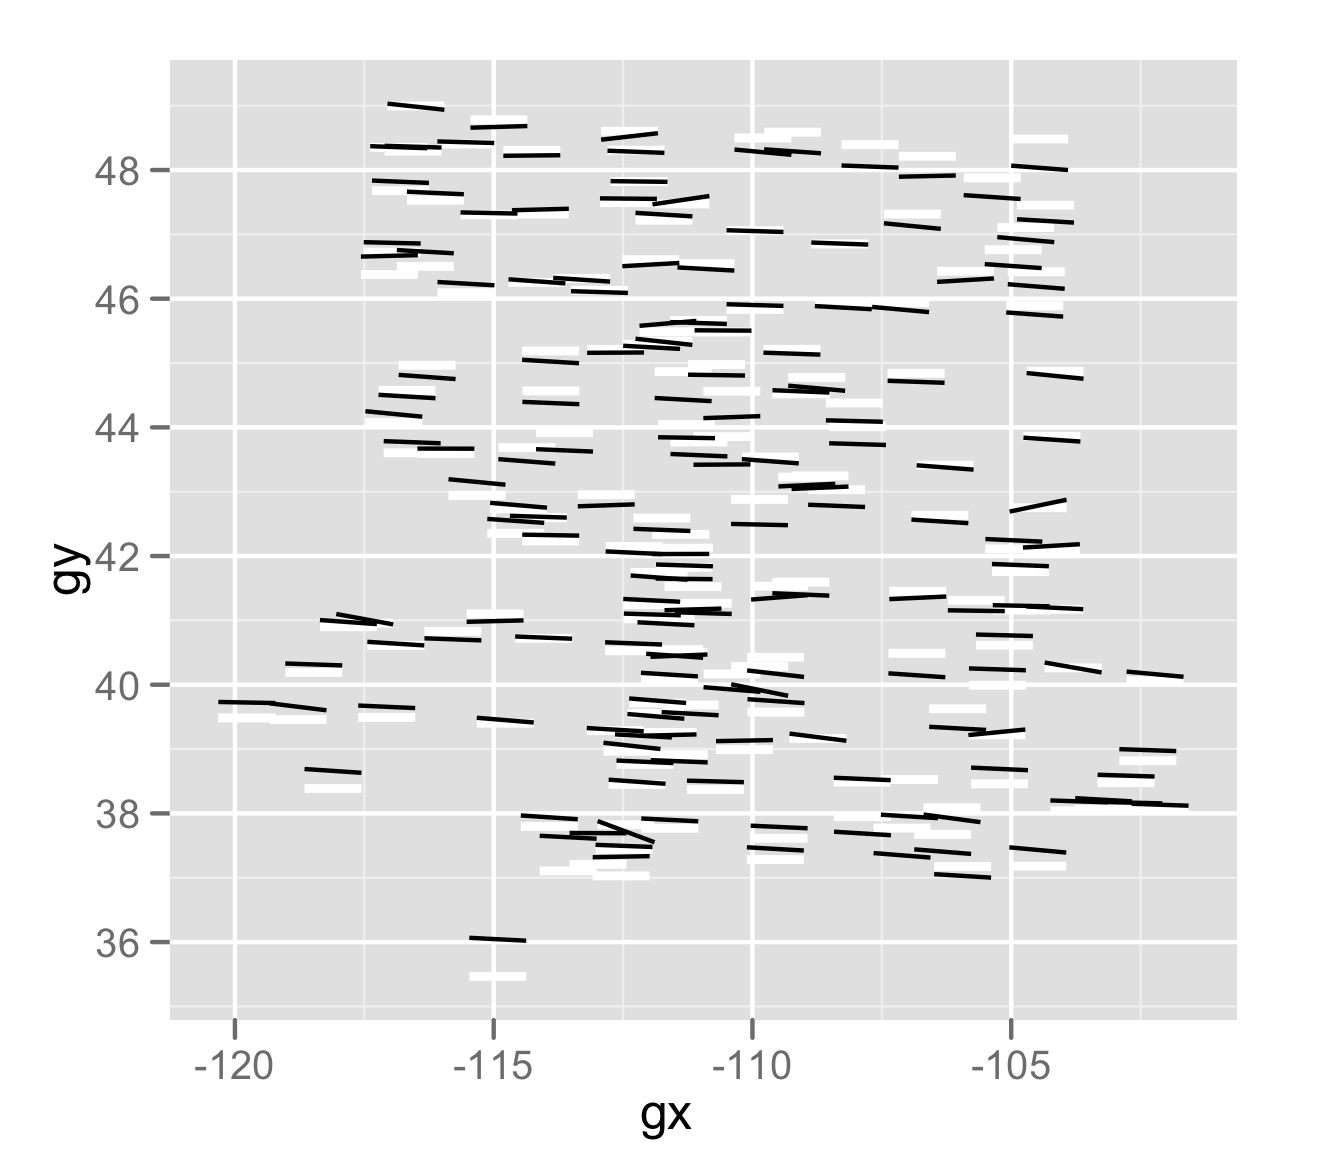
\includegraphics[width=0.25\linewidth]{ghcn-mountains}%
  \caption{(Top) Glyph-maps of the linear trend in ground station temperature values, 1950--2010, for USHCN stations, illustrating three issues for irregularly gridded data: overlapping icons, no natural choice for icon size, and the disordered appearance making comparisons more difficult. (Bottom) Legend showing
    temperature and temporal ranges of individual glyphs. }% (left) and stations in the mountain states (right).} 
  \label{fig:irregular}
\end{figure}
%The two panels illustrate one approach to the overlapping problem: zooming.  
One solution to the overlapping problem is to zoom in on smaller regions. There is an interplay between icon size (in geographical units), plotting area (in geographical units) and plot size (in display units).  Icons need to be big enough to be readable on the display, but small enough to avoid overlapping.  Readability can be maintained and overlapping reduced by decreasing the icon size and simultaneously increasing the display size or decreasing the plotting area.
% (as done in the right panel in Figure \ref{fig:irregular}).  
However, there are generally limitations in the maximum display size (or resolution) and the utility of plotting very small areas.  

An alternative approach is to combine overlapping locations and plot a single summary icon.  In Figure \ref{fig:irregular-collapsed} nearby locations are collapsed to a single icon.  In the top panel each station still has an individual glyph but locations close to each other share a plotting area.  Not all glyphs are suited to this kind of space sharing, another option is to perform a summary of the locations that are collapsed and display that instead of the raw data.  The bottom panel shows an example of this where the average trend for the collapsed locations is displayed.  It is helpful to differentiate glyphs that involve summaries of more than one location, here a heavier line indicates at least two locations have been averaged.  The aggregation of spatial locations to a single summary can be misleading.  The sensitivity of analyses to the scale and configuration of aggregation is described by the  modifiable areal unit problem (\cite{Openshaw:1984kx, Fotheringham:1991uq}). In this type of glyph map the scale of aggregation is determined, rather arbitrarily, by the icon size. This dependence of visual inferences on the icon size is undesirable.  The ability to interactively modify icon size, and zoom quickly to disaggregate locations would go some way to alleviating the problem.


\begin{figure}[htbp]
  \centering
  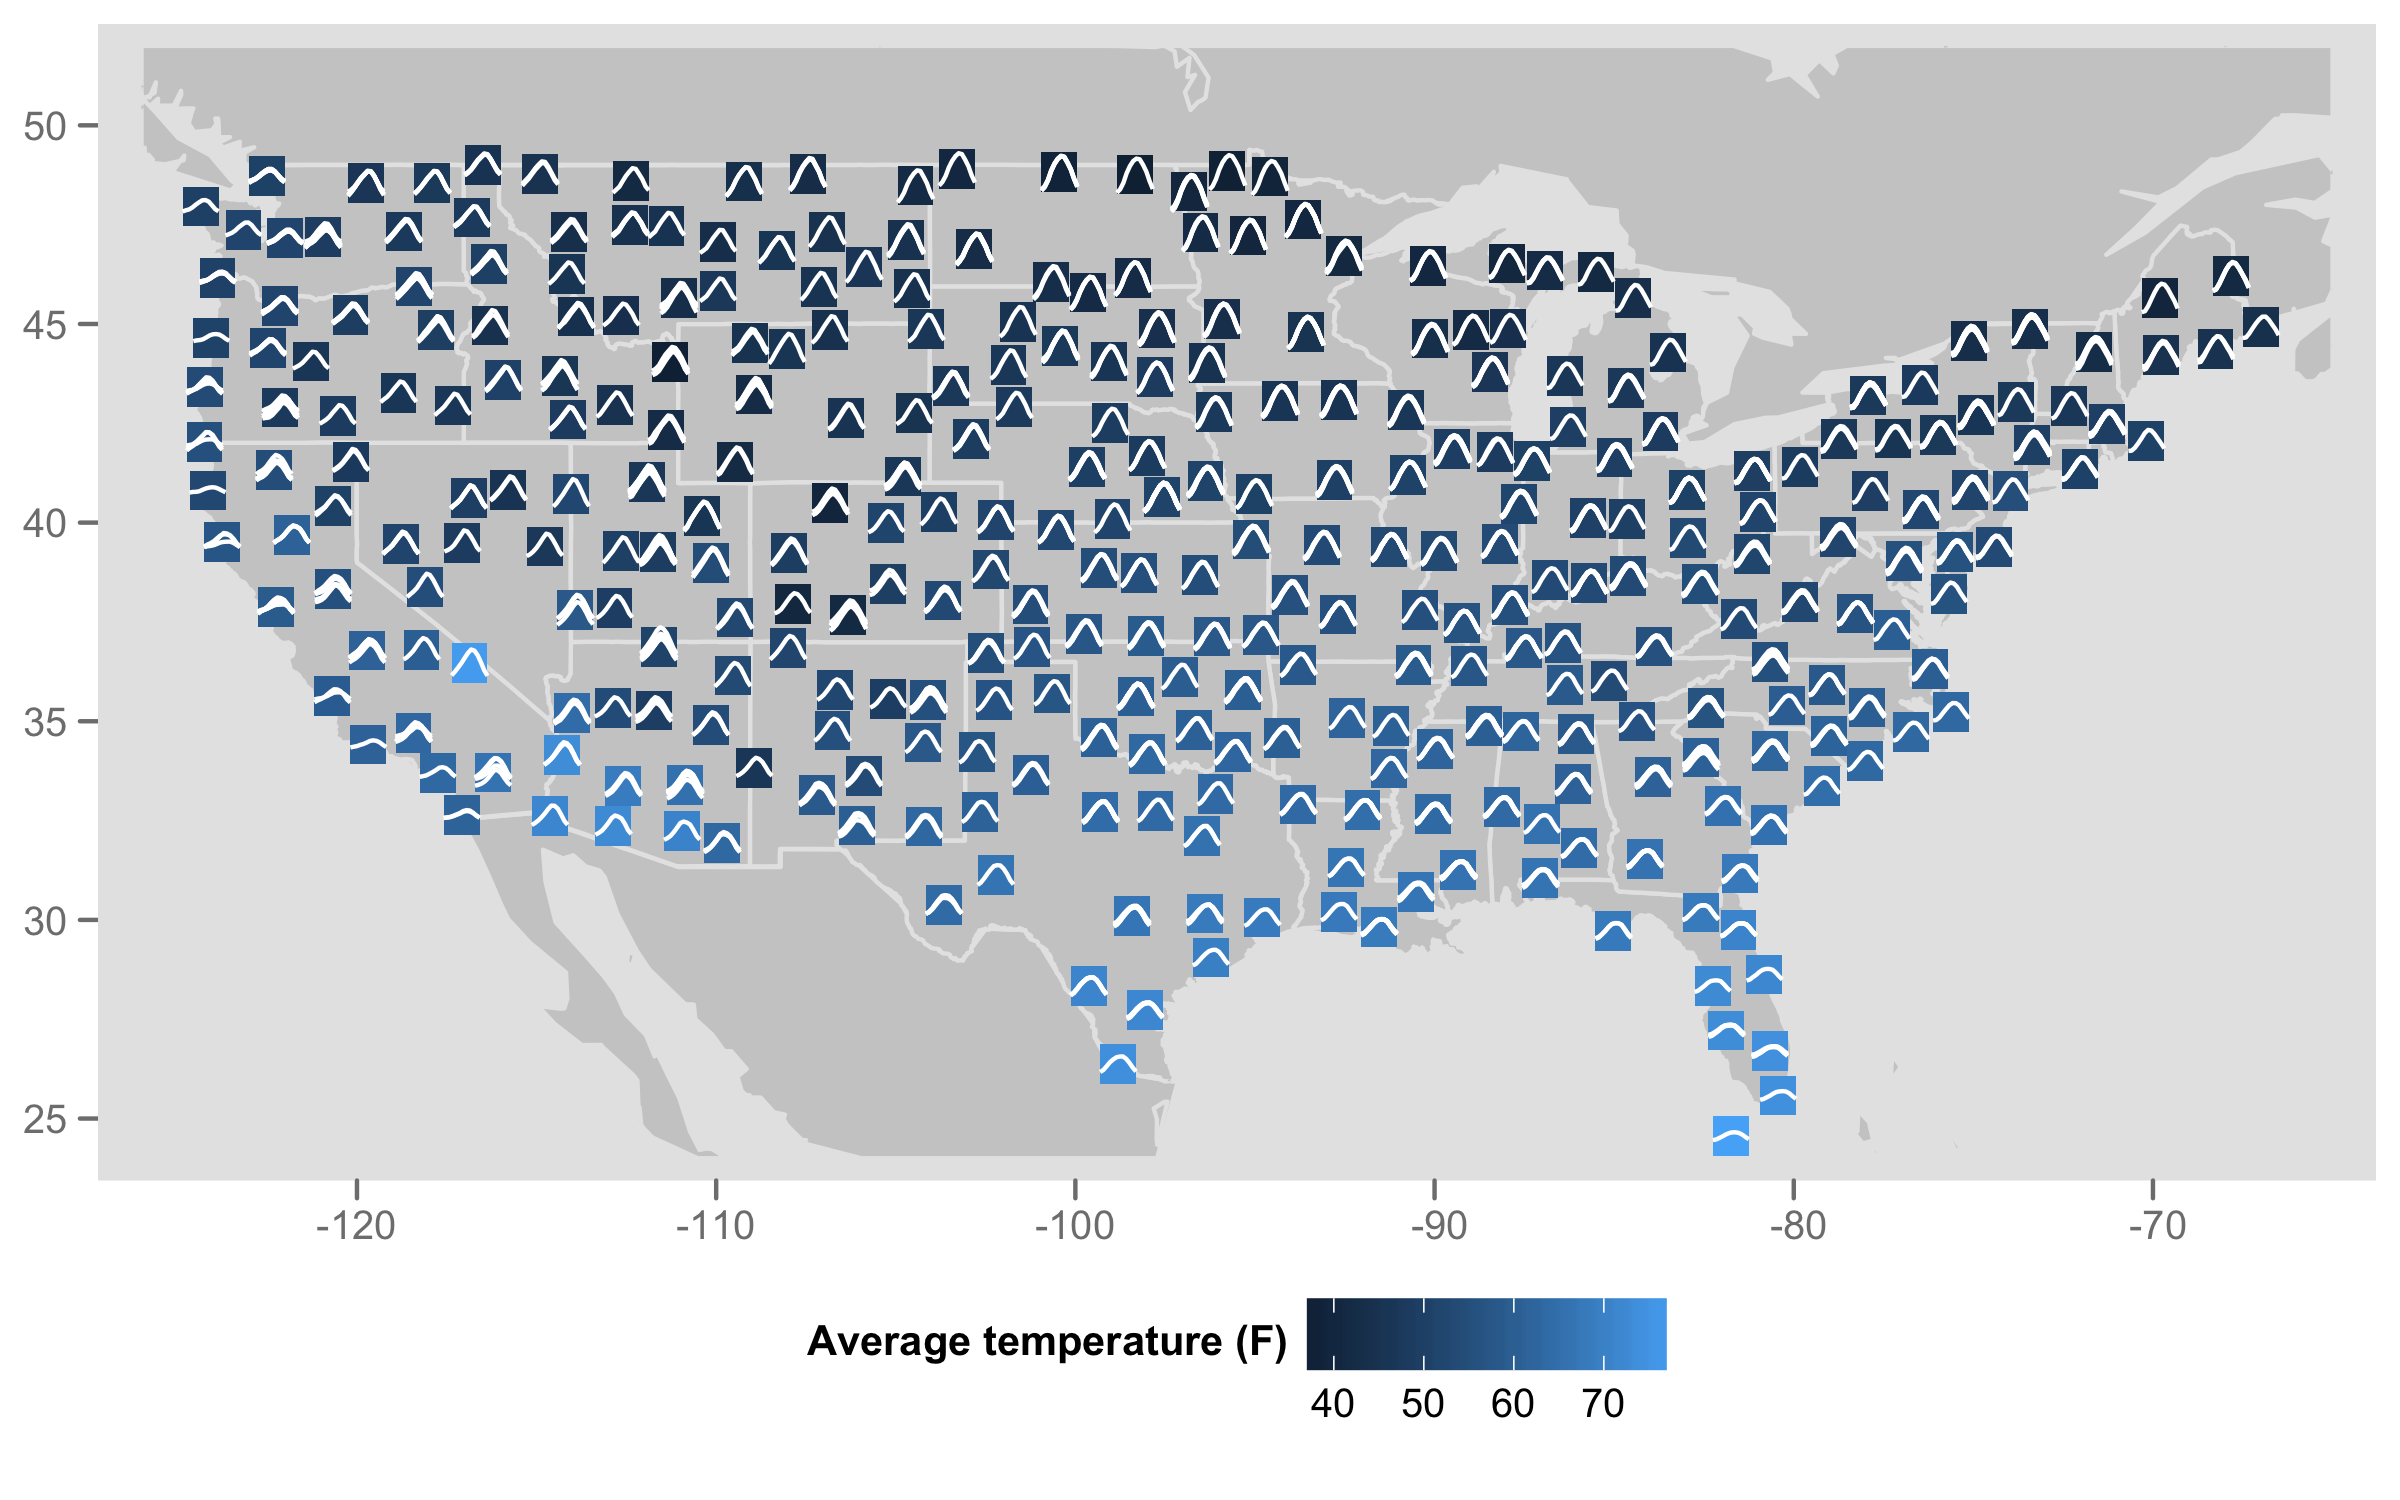
\includegraphics[width=0.5\linewidth]{usa-season-collapsed}%
  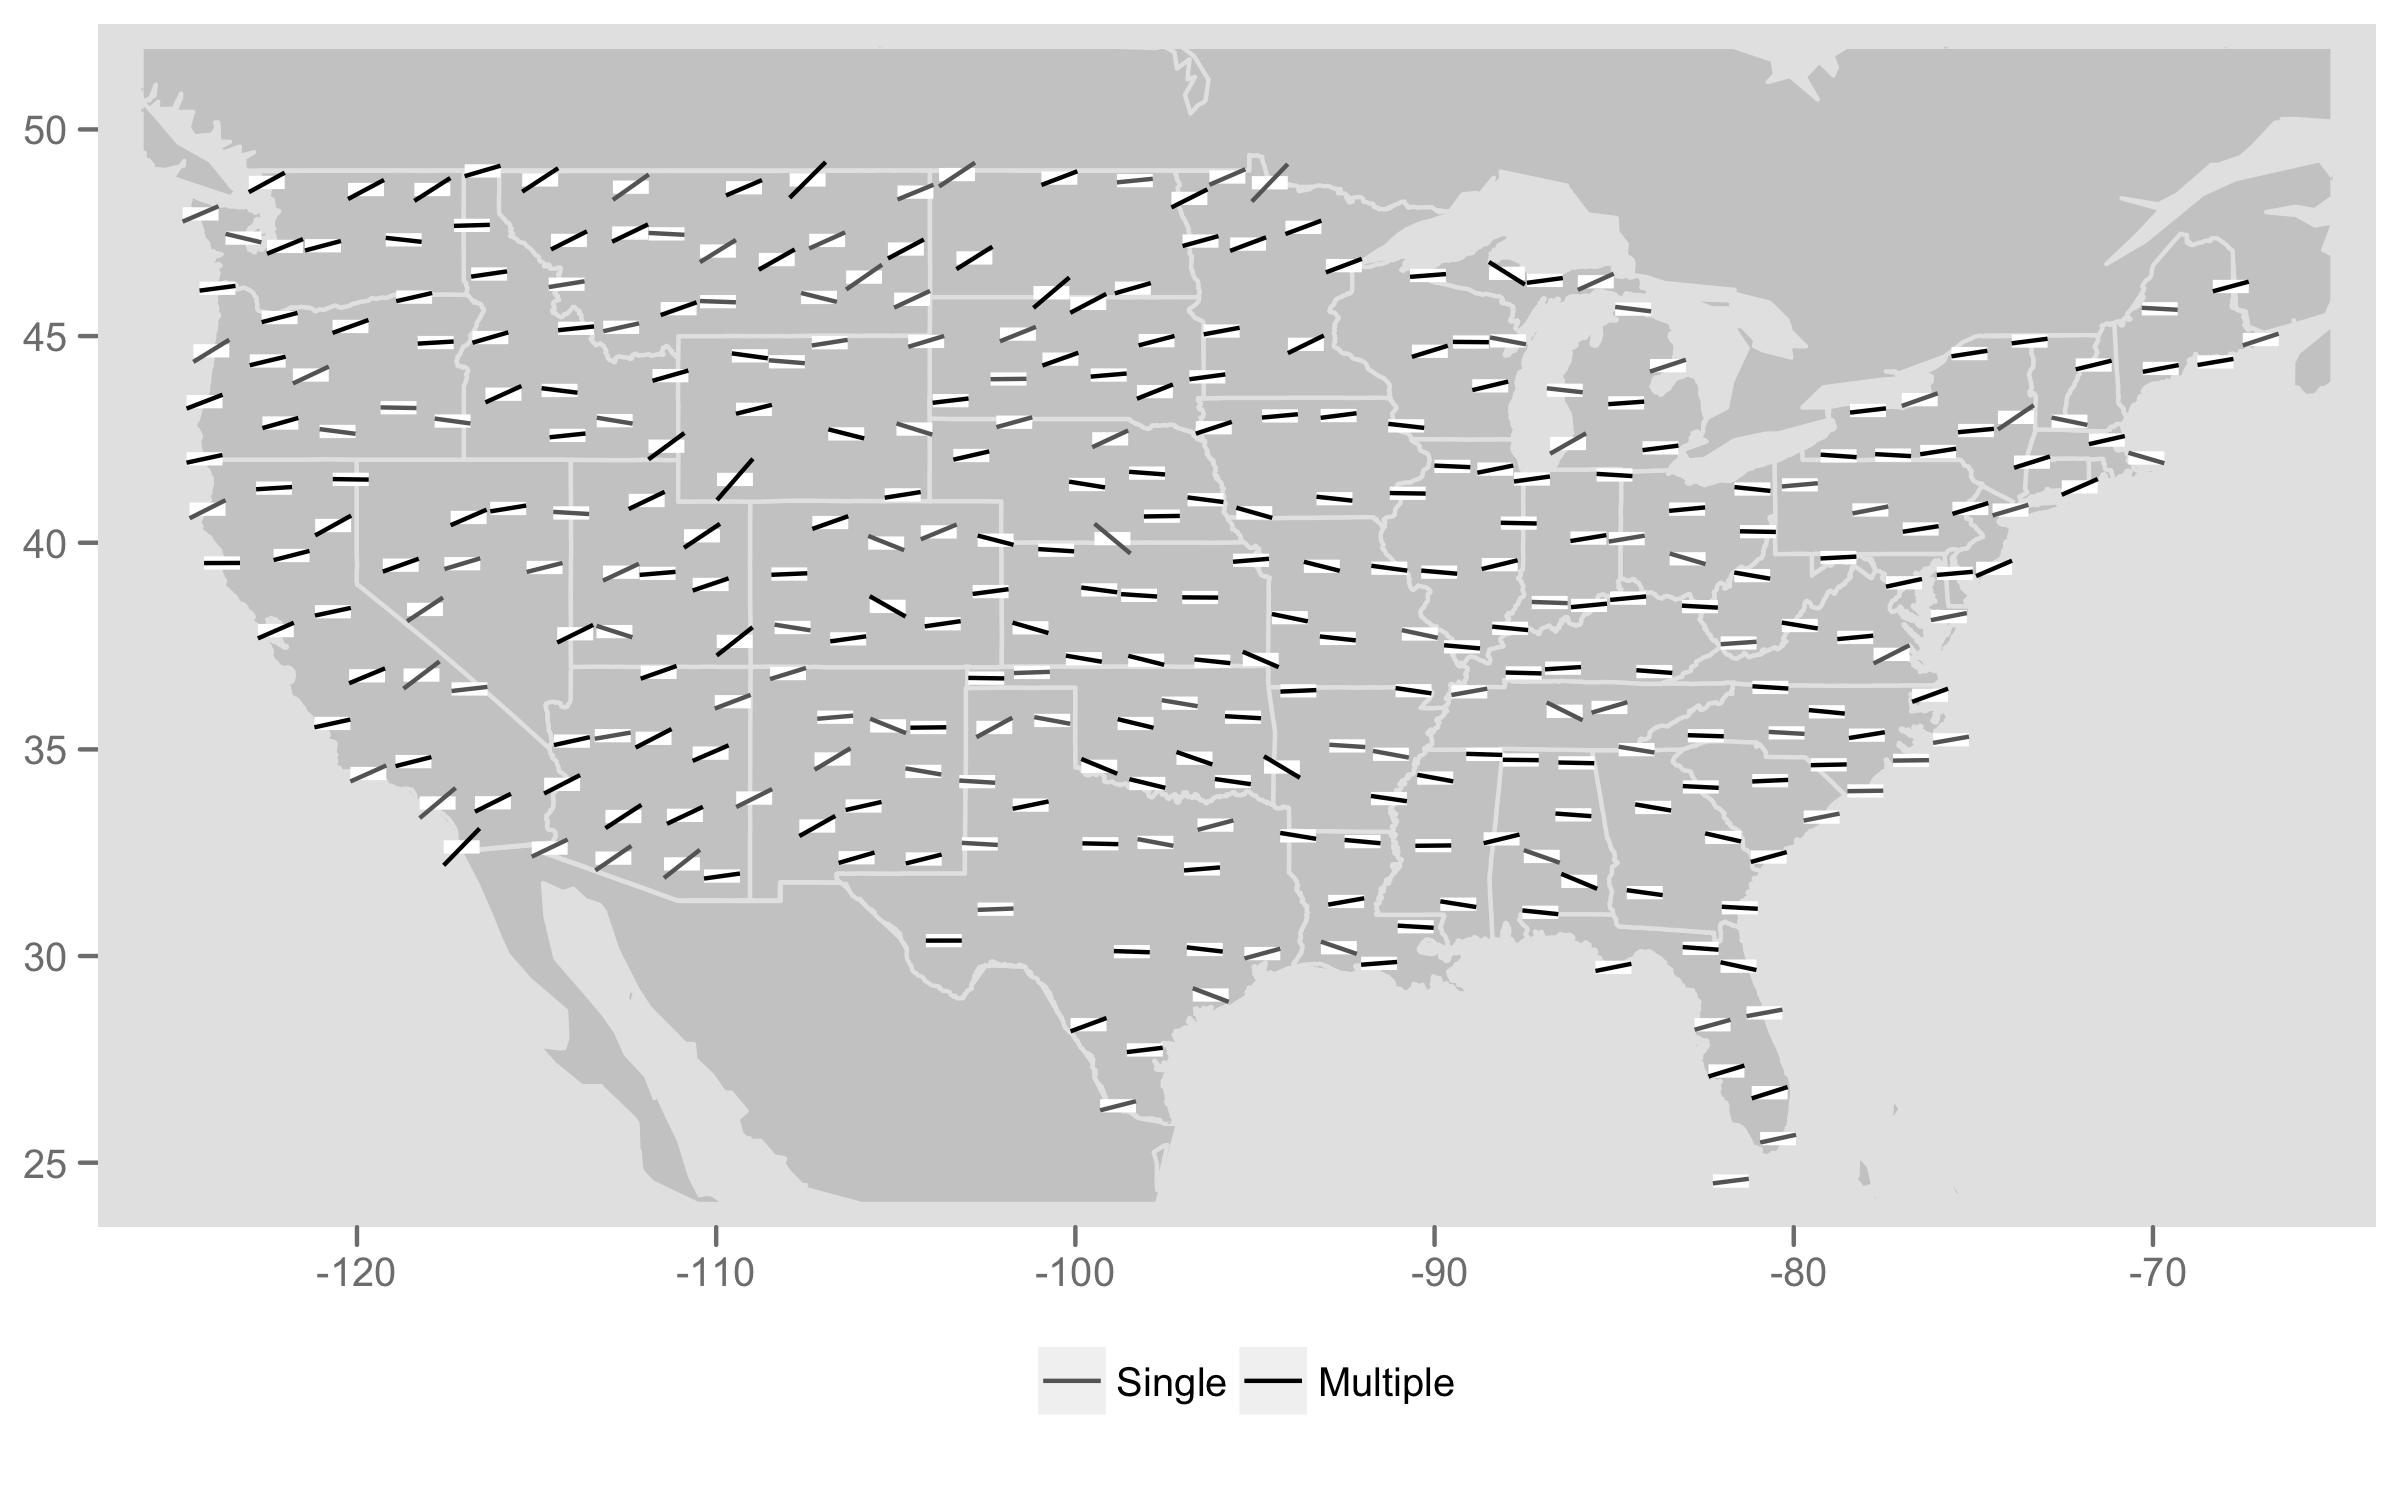
\includegraphics[width=0.5\linewidth]{usa-lin-collapse}%

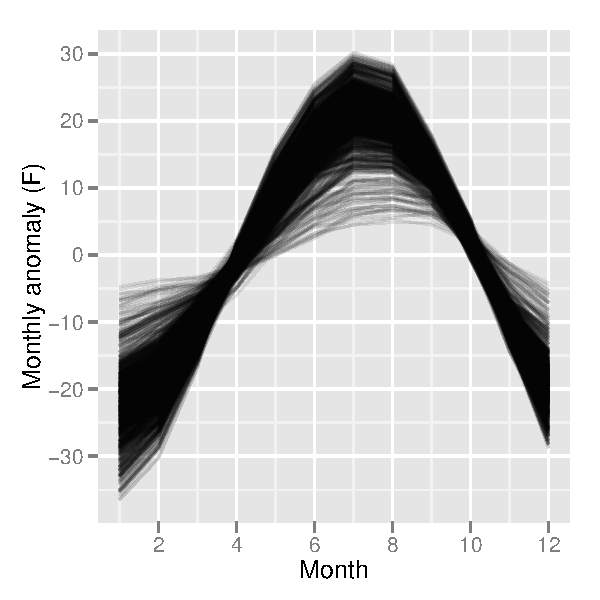
\includegraphics[width=0.20\linewidth]{usa-season-legend}\hspace{2in}%
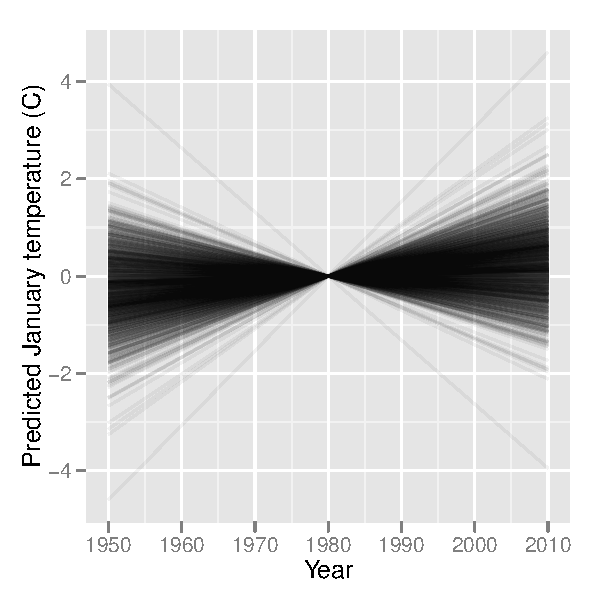
\includegraphics[width=0.20\linewidth]{usa-lin-legend}
  \caption{Glyph-maps of seasonal patterns (top left) and linear trends (top right) of USHCN stations, 1950--2010.  Nearby stations whose icons would overlap have been collapsed.  Each location has a glyph in the seasonal plot and color of the tiles corresponds to the average temperature of the locations.  Heavy lines in the linear trend plot correspond to average trends over more than one location. (Bottom) Legends showing scale of glyphs.} % Legend in Figure~\ref{fig:irregular-legend}}
  \label{fig:irregular-collapsed}
\end{figure}

In both examples of collapsing locations, the icon locations still represent real geographical locations of data, but contain data from up to an icon width away.  An alternative way to combine stations is to round locations to the icon size, Figure \ref{fig:irregular-grid}. This produces a regular grid with the advantage of easier perception of structure.  However, it hides the irregular nature of the locations and icons may end up centered over nonsense places (i.e. land measurements in the ocean).  

\begin{figure}[htbp]
  \centering
  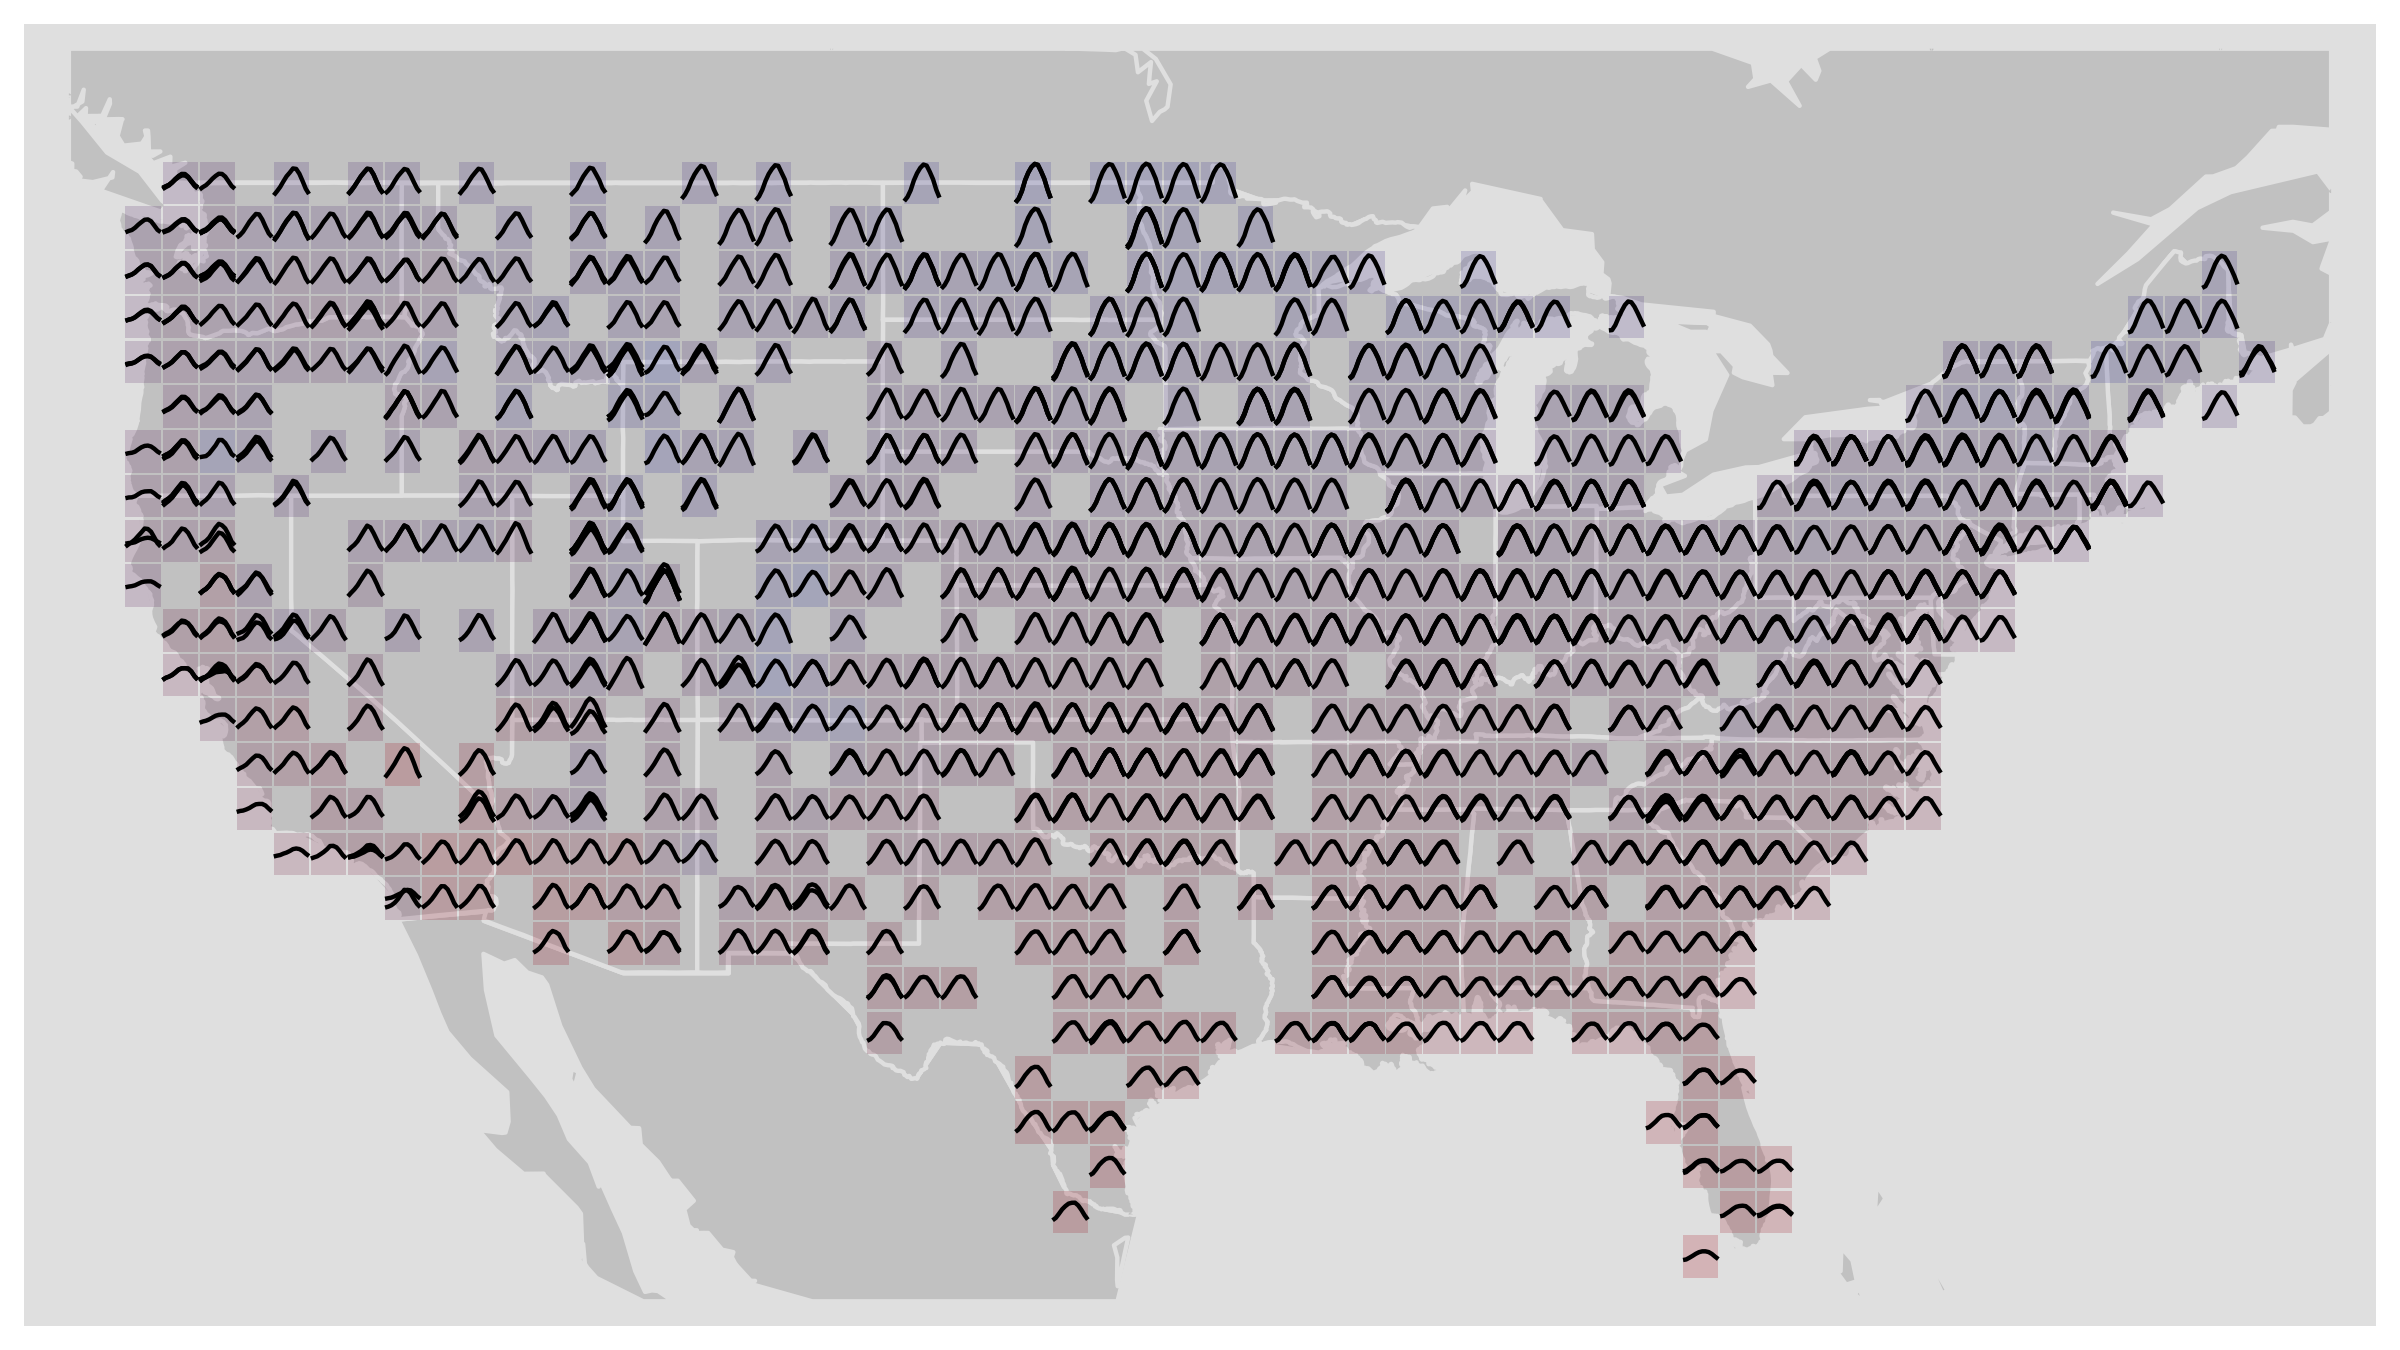
\includegraphics[width=0.5\linewidth]{usa-season-grid}%
  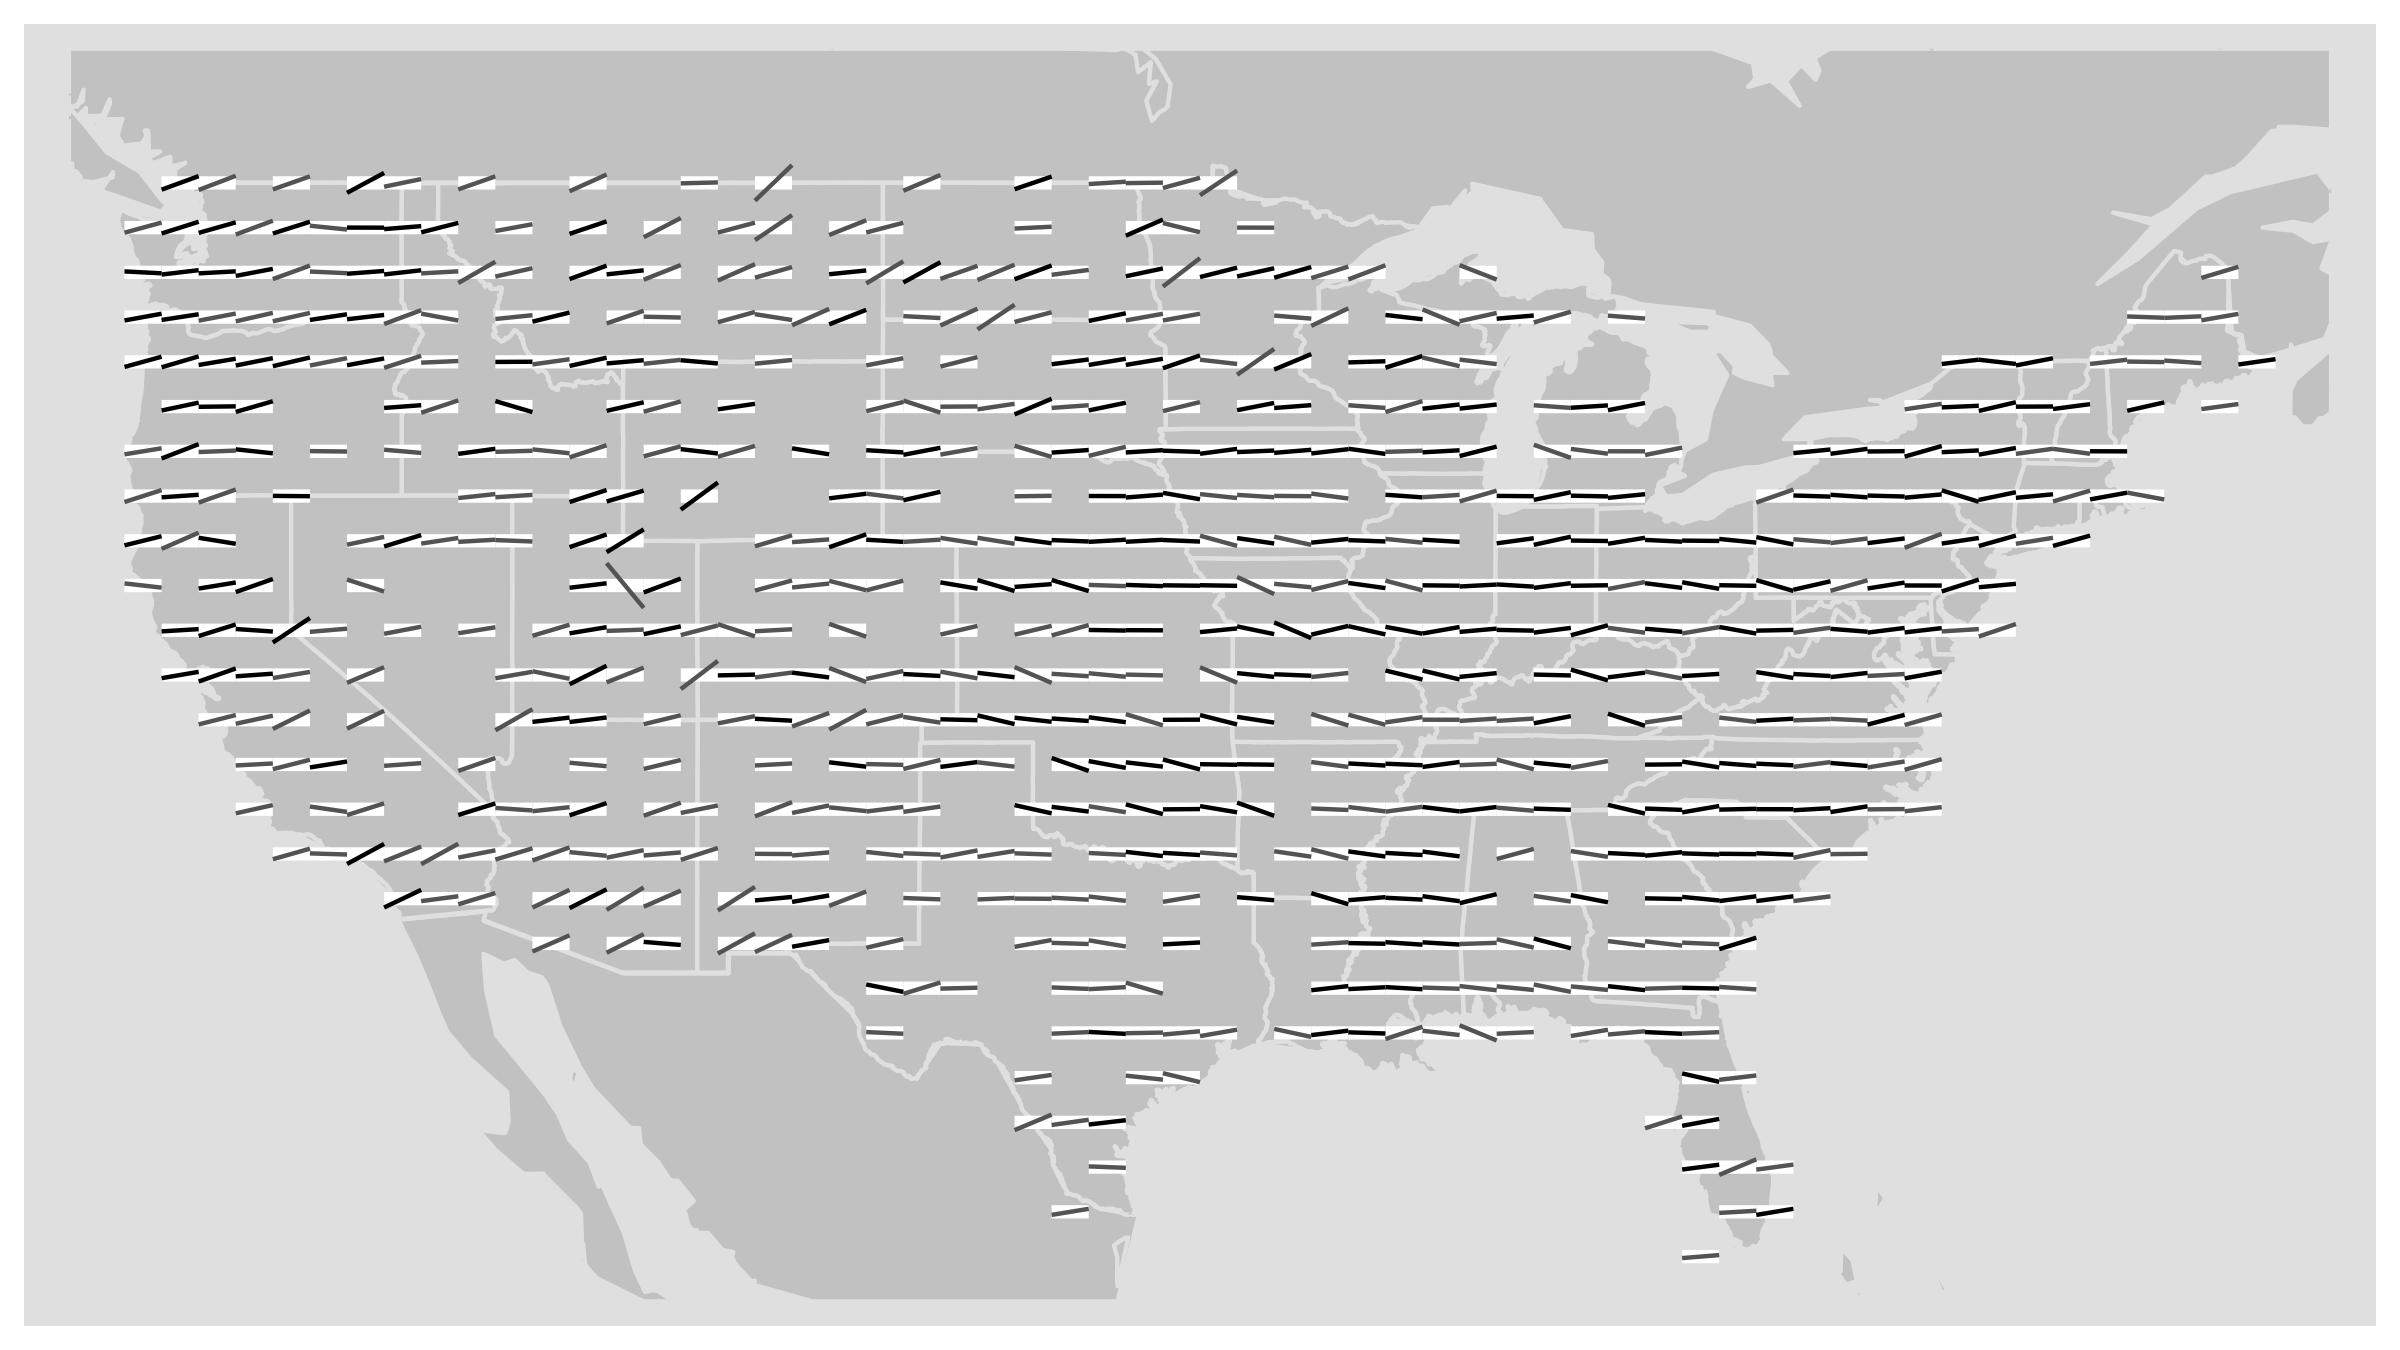
\includegraphics[width=0.5\linewidth]{usa-lin-grid}%

  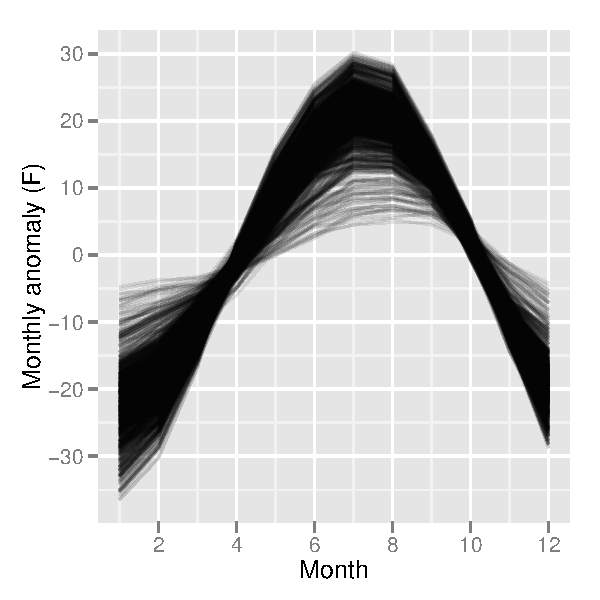
\includegraphics[width=0.20\linewidth]{usa-season-legend}\hspace{2in}%
  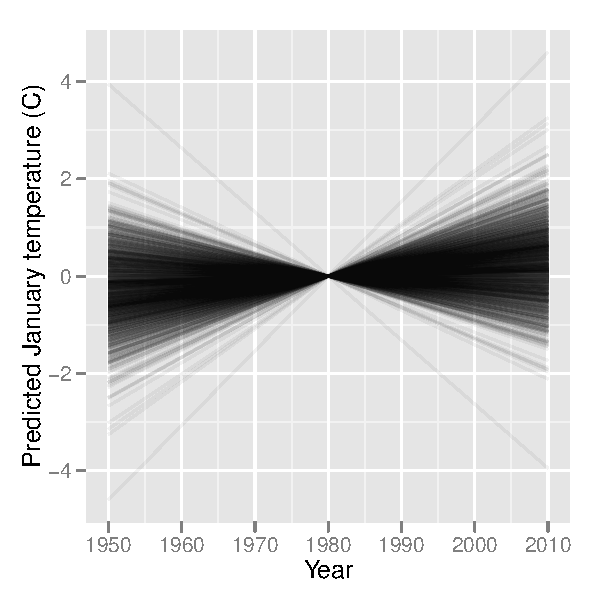
\includegraphics[width=0.20\linewidth]{usa-lin-legend}
  \caption{Glyph-maps of seasonal patterns (top left) and linear trends (top right) of USHCN stations, 1950--2010.  Station locations have been rounded to the nearest degree Each location has a glyph in the seasonal plot and color of the tiles corresponds to the average temperature of the locations. Heavy lines in the linear trend plot correspond to average trends over more than one location. (Bottom) Legends showing scale of glyphs.} %Legend in Figure~\ref{fig:irregular-legend}}
  \label{fig:irregular-grid}
\end{figure}

%\begin{figure}[htbp]
%  \centering
%  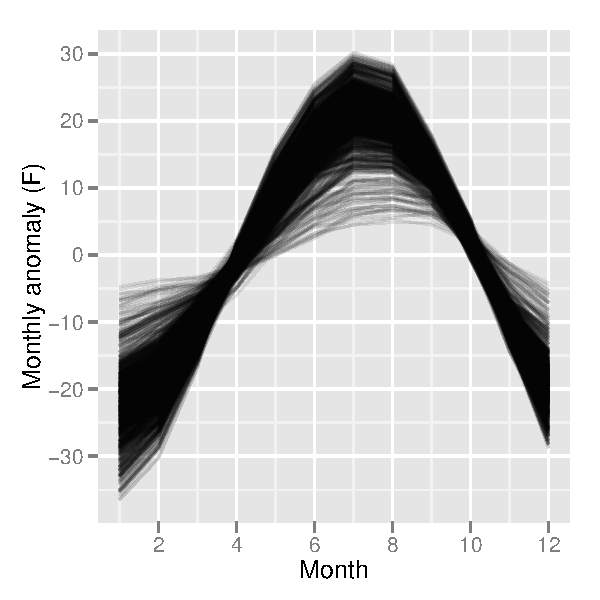
\includegraphics[width=0.33\linewidth]{usa-season-legend}%
%  \hspace{0.18 \linewidth}%
%  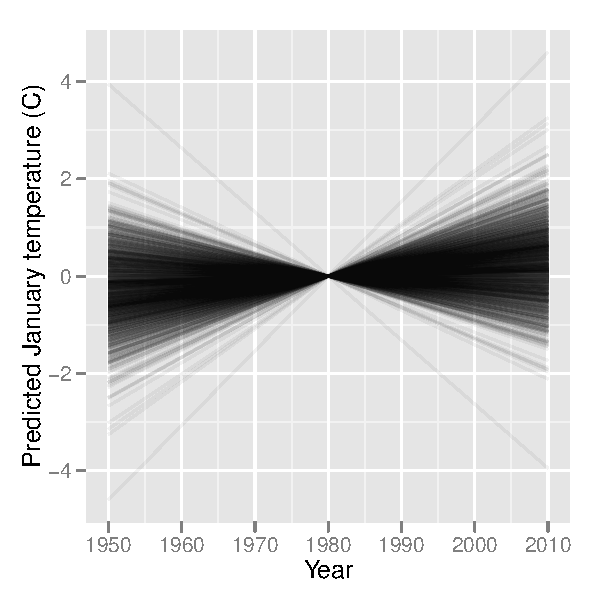
\includegraphics[width=0.33\linewidth]{usa-lin-legend}
  
%  \caption{Legend for Figures~\ref{fig:irregular-collapsed} aad \ref{fig:irregular-grid}.}
%  \label{fig:irregular-legend}
%\end{figure}

Reference guides become especially important in the irregular location case. Comparisons are harder in this case, as the ability to easily compare icons along a common baseline, be it along a row or column of glyphs, is absent. Without reference it is hard to tell if short series are missing data at the start or end.  

\begin{figure}[htbp]
  \centering
  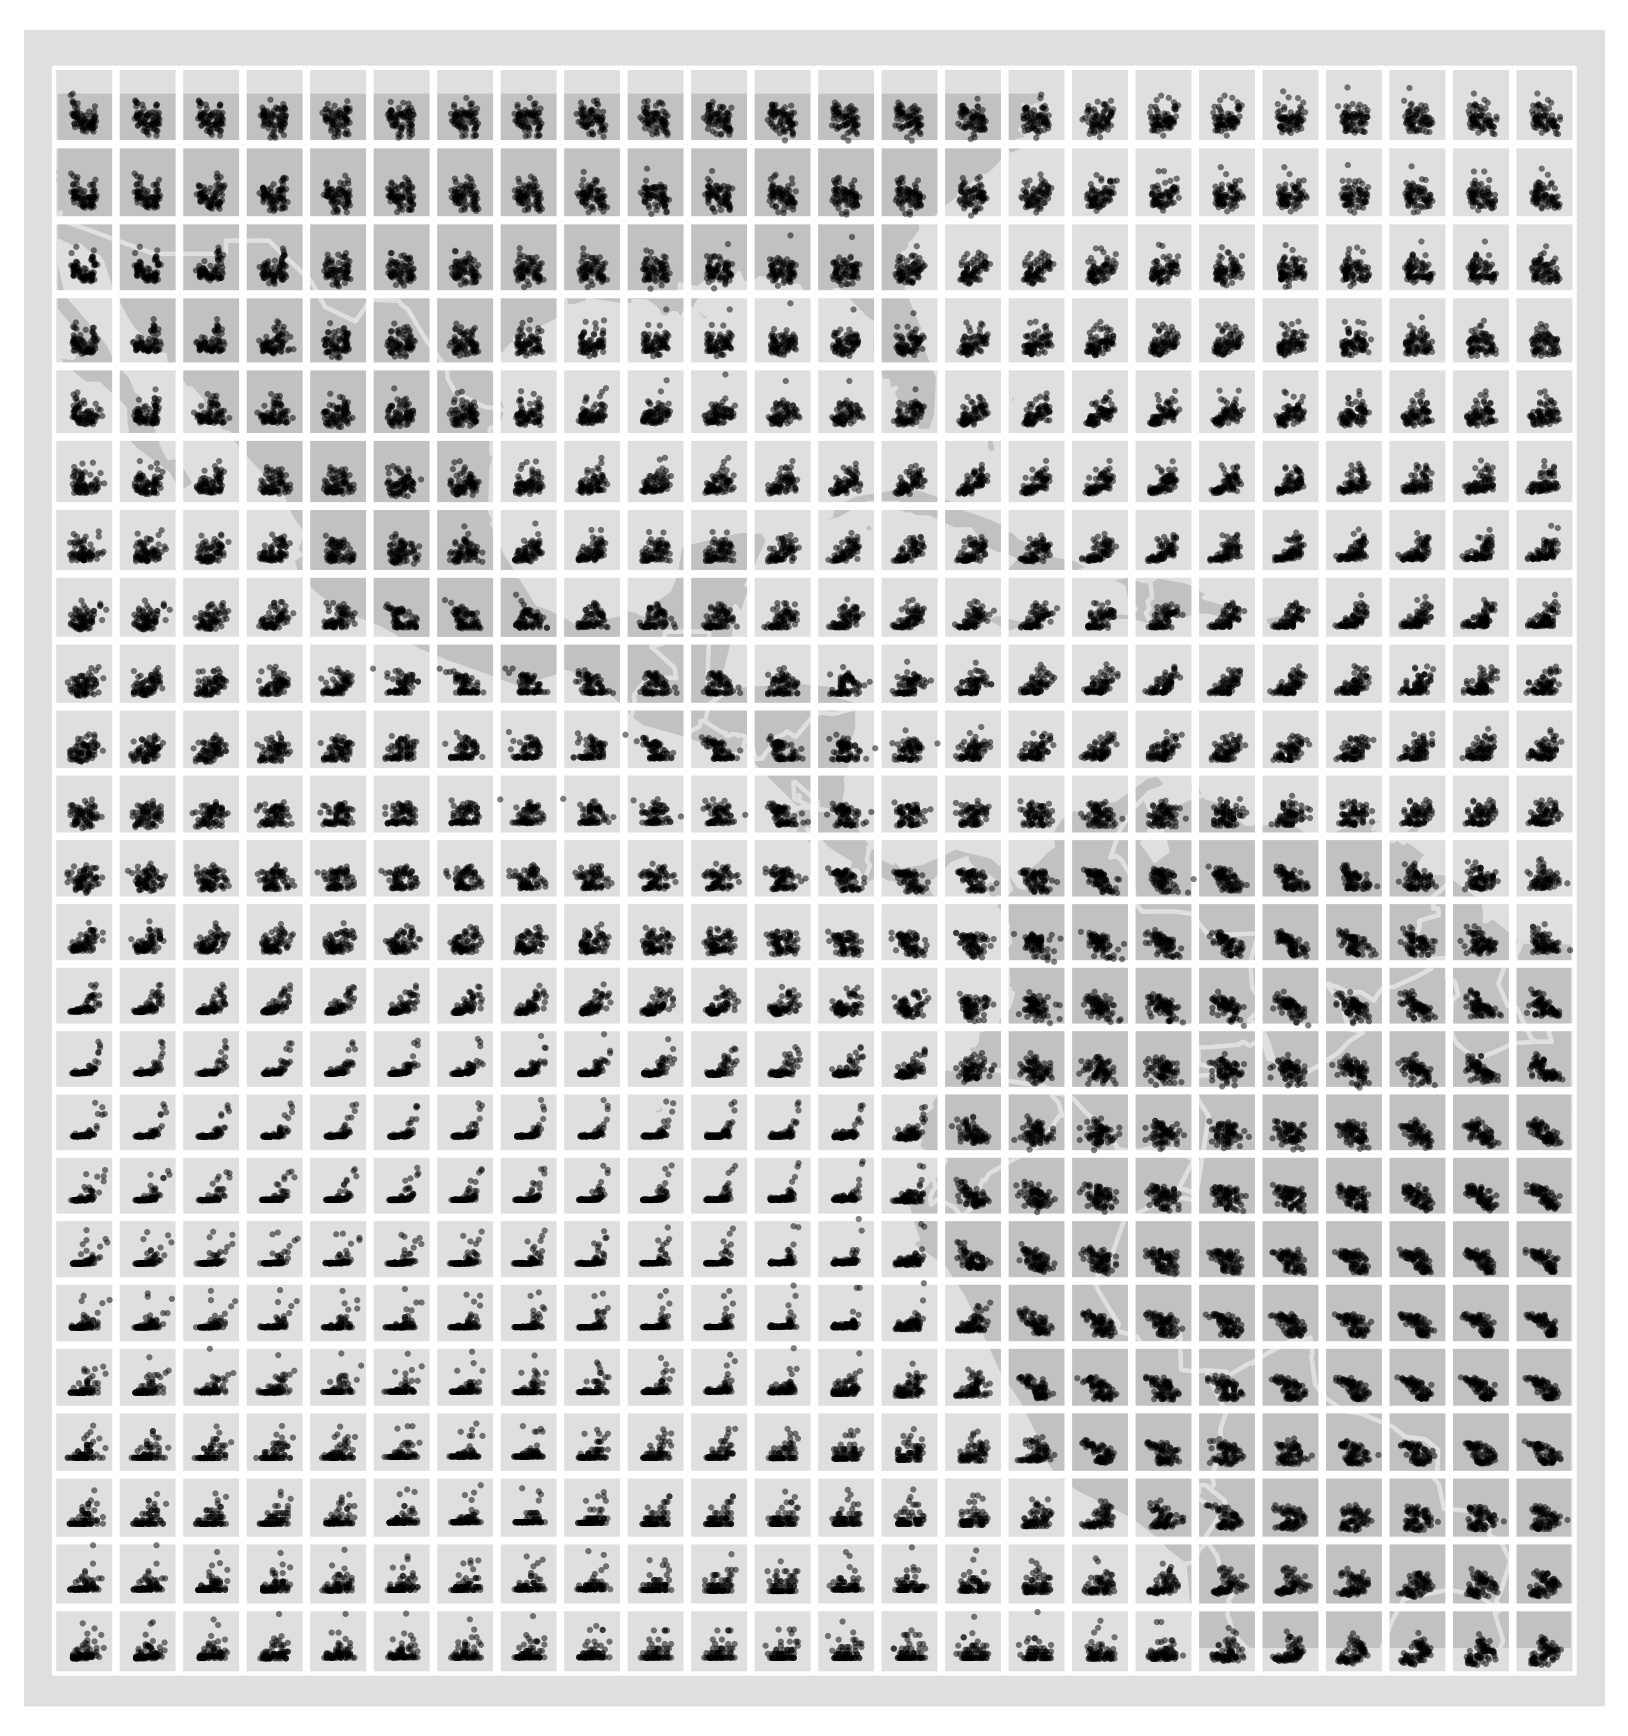
\includegraphics[width=0.5\linewidth]{nasa-scat-glyph}%
  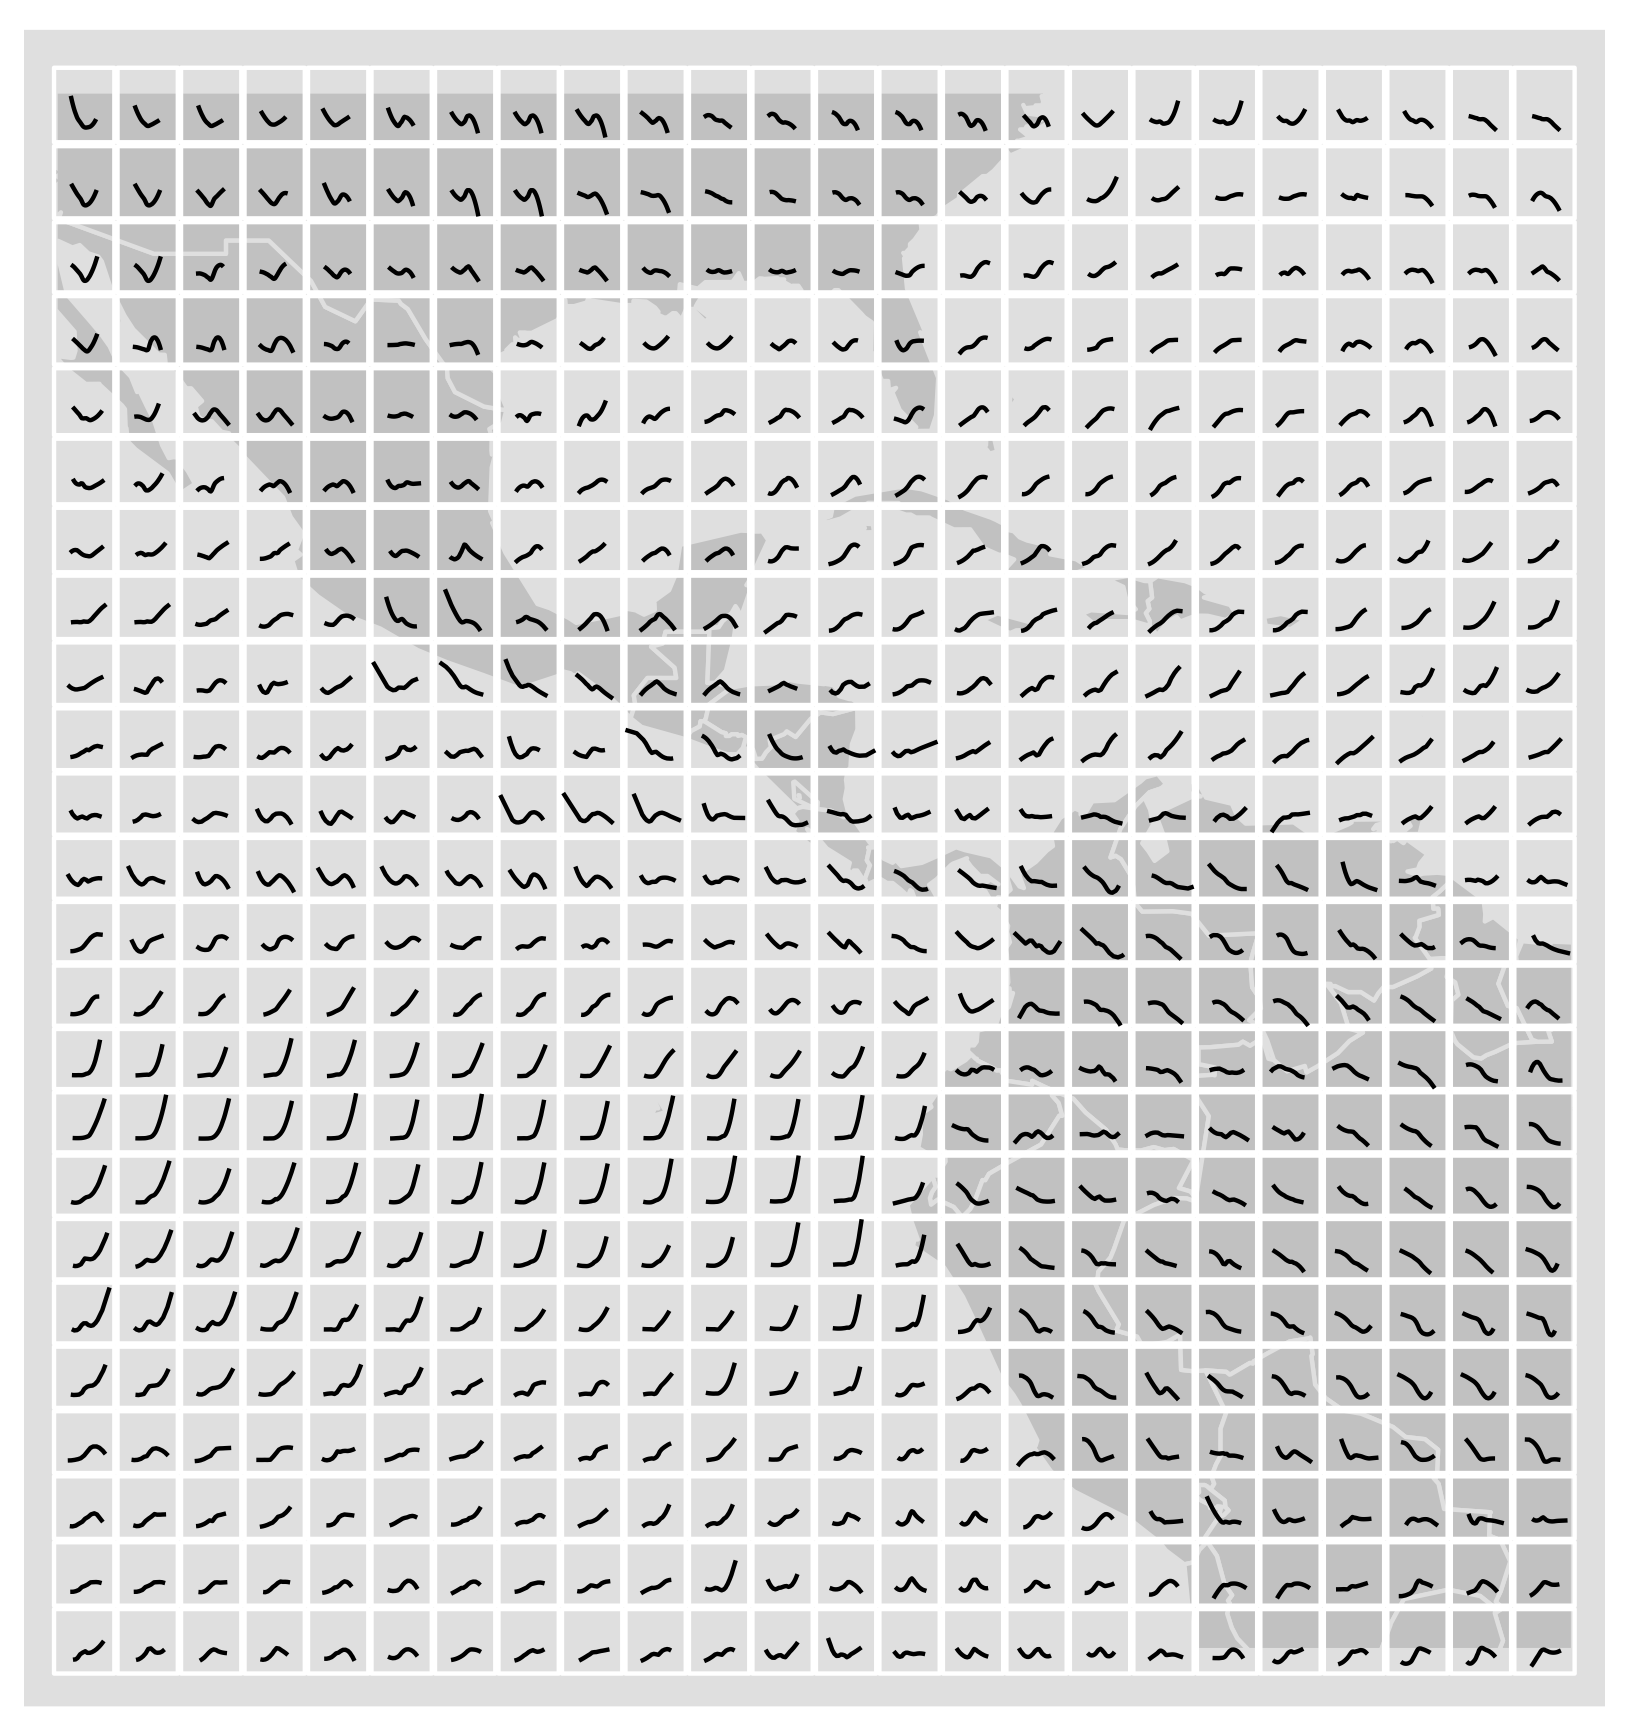
\includegraphics[width=0.5\linewidth]{nasa-loess-glyph}

  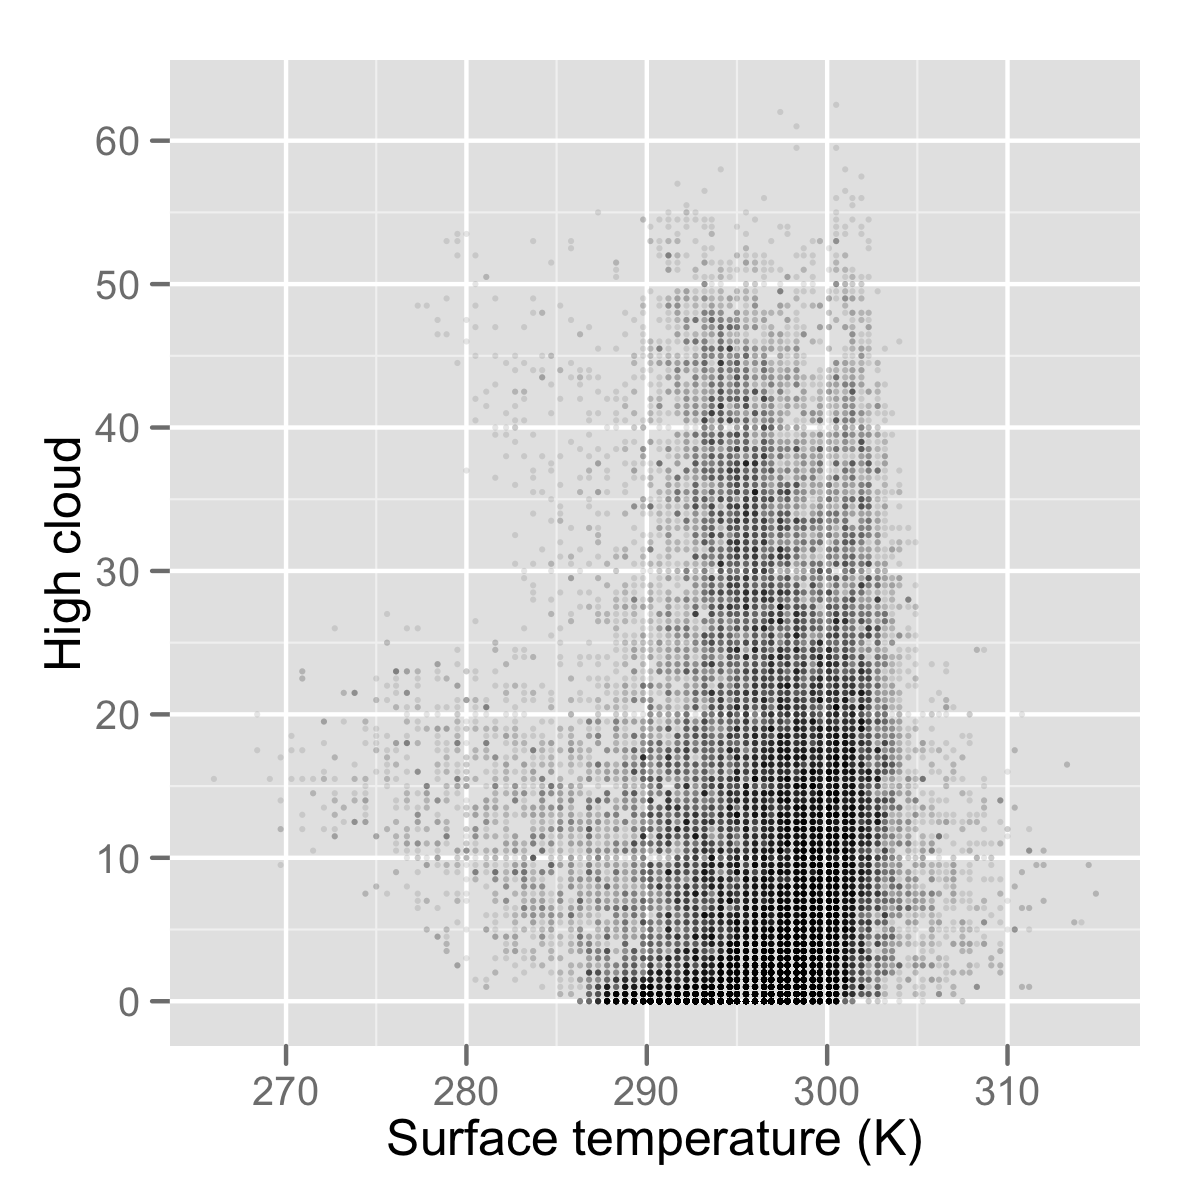
\includegraphics[width=0.20\linewidth]{nasa-scat-legend}%
  \hspace{0.17\linewidth}%
  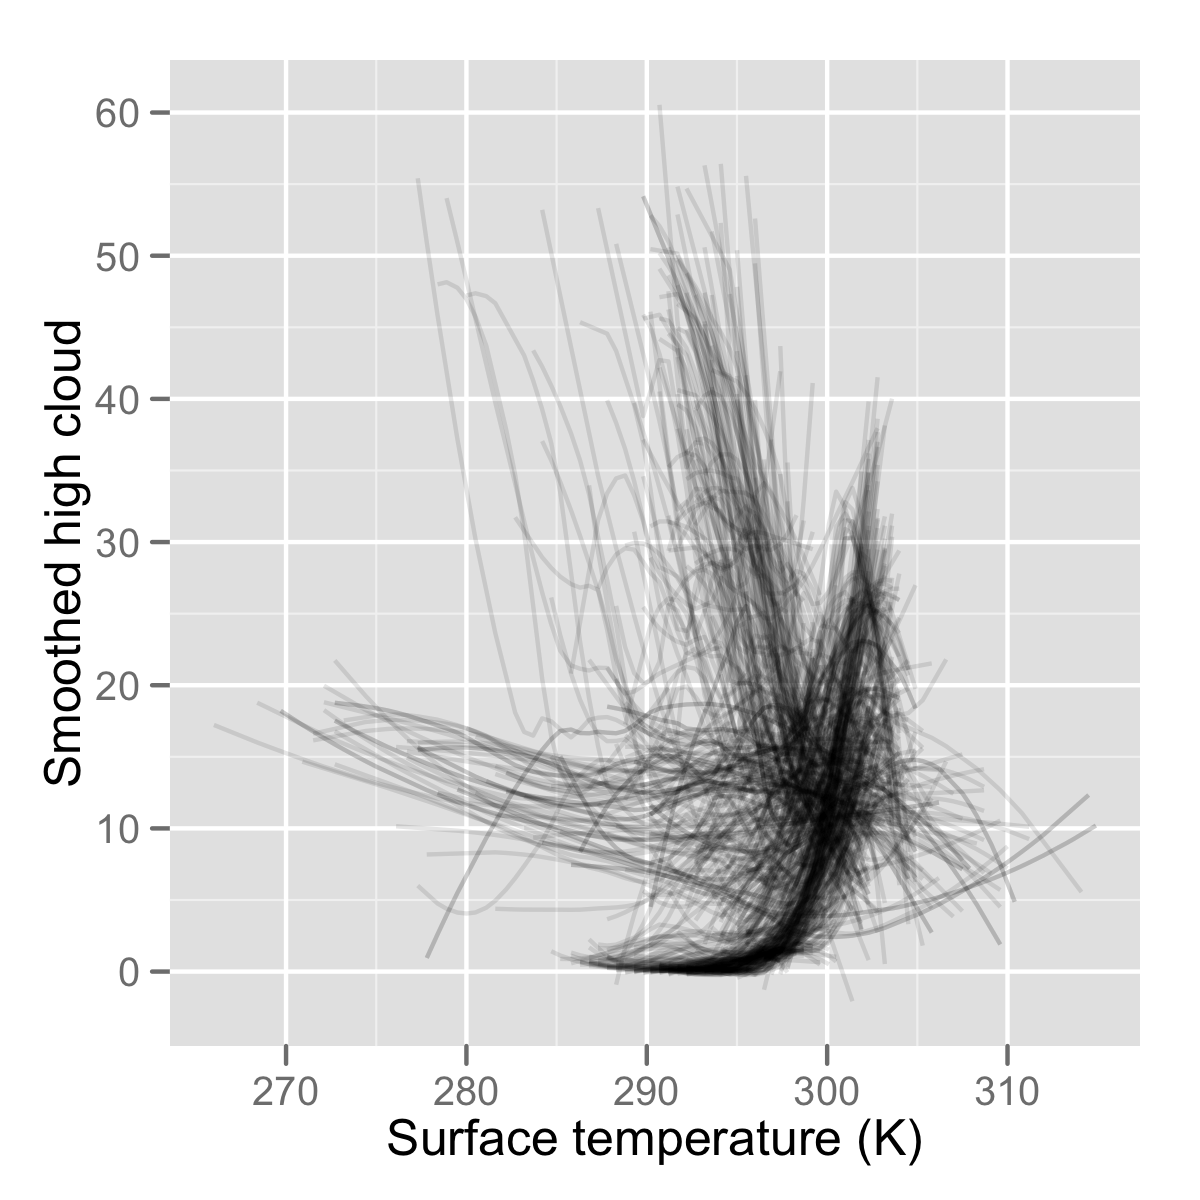
\includegraphics[width=0.20\linewidth]{nasa-loess-legend}

  \caption{Glyph-map showing (top left) scatterplot of temperature vs high-cloud and (top right) smoothed (loess) curve fit to each location. The relationship between these two variables varies considerably over the spatial domain. (Bottom) Legends show overall patterns and scales.}
  \label{fig:cloud}
\end{figure}

\section{Generalizations}

Glyphs can be more general than time series or stars. For multivariate data we may want to represent several variables in the glyphs. Figure~\ref{fig:cloud} shows scatterplots of the EXPO data as icons: temperature values are displayed horizontally and high-cloud values are displayed vertically, both locally scaled. The bivariate relationship between the two variables is explored spatially, and it is clear that it is different across the region. The equatorial Pacific and Caribbean have positive association between temperature and high cloud, while the south American continent has negative association. The second plot displays a loess curve fit to the data instead of the individual points, sharpening the view of association. Another option is available in Gauguin \citep{gribov:2006}, a icon based on a histogram, giving small univariate distribution displays for each location.

\section{Discussion}

There are two natural next directions for this work: perceptual experiments, and development of interactive graphics. Several careful studies comparing the perceptual elements of these displays, using different scale and glyph options, and in comparison with facetted heatmaps, would be recommended. For example, it appears that periodic trends are easier to perceive in star-glyphs, and long-term trends in line-glyphs. Is this always the case? Are their certain types of periodicity that are particularly easy to spot? These questions need to be answered with rigorous perceptual studies to help guide the use of these plots.

The conceptualization and equations for computing the glyph-maps lend themselves to producing these displays interactively. Different variables can be swept into the display using mouse motion, resolution could be increased upon zooming in to a spatial neighborhood. This experimentation is ideally done using R, so that computation can be linked with displays. The hurdle is the lagging development of interactive graphics in R. Several new packages that support interactive graphics in R have become available in the past year \citep{qtbase, qtpaint, plumbr} which will enable these experiments.

In summary, glyph-maps enable the study of temporal patterns in multivariate spatiotemporal data. Climate change is focused on changes over time, so glyph-maps provide a way to study these changes directly. Glyph-maps enable different resolutions of the data to be examined: the raw data to discover data quality issues, early, global trend, seasonality, residuals, and multivariate dependencies. When the data is spatially gridded the glyphs are organized in a manner that makes reasonable comparisons. For irregularly gridded data the icon size needs to be chosen to minimize overlap but use as much display space as possible, or combined to produce close to gridded icons. 



\bibliography{references}

\end{document}